\RequirePackage[l2tabu, orthodox]{nag}	% keep on nagging
\makeatletter
\renewcommand\thenag@c{\romannumeral\c@nag@c}
\makeatother


\documentclass[a4paper,twoside,10pt]{report}
% Alternative Options:
% Duplex: oneside / twoside
% Base Font Size: 10pt / 11pt / 12pt

%%%%%%%%%%%%%%%%%%%%%%%%%%%%%%%%%%%%%%%%%%%%%%%%%%%%%%%%%%%%%
%% Options / Modifications / Packages
%%%%%%%%%%%%%%%%%%%%%%%%%%%%%%%%%%%%%%%%%%%%%%%%%%%%%%%%%%%%%


%%%%%%%%%%%%%%%%%%%%%%%%%%%%%%%%%%%%%%%%%%%%%%%%%%%%%%%%%%%%%
%% Layout
%%%%%%%%%%%%%%%%%%%%%%%%%%%%%%%%%%%%%%%%%%%%%%%%%%%%%%%%%%%%%

\usepackage{geometry}
\usepackage{lipsum}
\geometry{a4paper,left=40mm,right=30mm, top=2cm, bottom=3cm}
\oddsidemargin=-1cm
\setlength{\textwidth}{16cm}
\setlength{\textheight}{22cm}
\setlength{\headheight}{12.6pt}
\setlength{\topmargin}{0pt}
\setlength{\oddsidemargin}{8mm}



%% Language %%%%%%%%%%%%%%%%%%%%%%%%%%%%%%%%%%%%%%%%%%%%%%%%%
\usepackage[T1]{fontenc}		% font encoding
\usepackage[utf8]{inputenc}		% input encoding
\usepackage{lmodern}			% fonts
\usepackage[naustrian,greek,english]{babel}
\selectlanguage{english}


%% Packages for Graphics & Figures %%%%%%%%%%%%%%%%%%%%%%%%%%

% use predefined colours
% see http://en.wikibooks.org/wiki/LaTeX/Colors
\usepackage[usenames,dvipsnames]{xcolor} % provides colours
% define some colors
\definecolor{dkgreen}{rgb}{0,0.6,0}
\definecolor{mauve}{rgb}{0.58,0,0.82}
\definecolor{DarkGrey}{rgb}{0.1,0.1,0.1}
\definecolor{magenta}{rgb}{0.79216,0.12156,0.48236}

\usepackage[pdftex]{graphicx}
\usepackage{tikz,pgfplots}		% provides TikZ
\usepackage{epstopdf}
\usepackage{afterpage}
\usepackage{emptypage}
%\pgfplotsset{compat=1.10}
%\usetikzlibrary{arrows.meta}


% variables used with matlab2tikz
\newlength\figureheight
\newlength\figurewidth

% introduce the file extension *.1 to latex
\DeclareGraphicsRule{.1}{mps}{.1}{}

\usepackage{subfig}				% provides subfloat



%%%%%%%%%%%%%%%%%%%%%%%%%%%%%%%%%%%%%%%%%%%%%%%%%%%%%%%%%%%%%
%% Mathematics
%%%%%%%%%%%%%%%%%%%%%%%%%%%%%%%%%%%%%%%%%%%%%%%%%%%%%%%%%%%%%


%% Math Packages %%%%%%%%%%%%%%%%%%%%%%%%%%%%%%%%%%%%%%%%%%%%
\usepackage{amsmath}
\usepackage{amsthm}
\usepackage{amsfonts}
\usepackage{amssymb}

\usepackage[squaren]{SIunits}	% provides \metre, etc.


%% Nomenclature %%%%%%%%%%%%%%%%%%%%%%%%%%%%%%%%%%%%%%%%%%%%%
\usepackage[intoc]{nomencl}
\makenomenclature

% D	dimensionless numbers: 		symbol, description, definition
% G	Greek symbols				symbol, description, unit
% L	Latin (Roman) symbols		symbol, description, unit
% X	Other?						symbol, description, unit
% U	subscripts					symbol, description
% S	superscripts				symbol, description
% O	oversymbols					symbol, description

%\setlength{\nomitemsep}{-\parsep}
   \RequirePackage{ifthen}
   \renewcommand{\nomgroup}[1]{%
     \ifthenelse{\equal{#1}{G}}{\item[]\item[\Large\textbf{Greek Symbols}]}{%
       \ifthenelse{\equal{#1}{L}}{\item[]\item[\Large\textbf{Latin Symbols}]}{%
         \ifthenelse{\equal{#1}{D}}{\item[]\item[\Large\textbf{Dimensionless Groups}]}{
         	\ifthenelse{\equal{#1}{X}}{\item[]\item[\Large\textbf{Other Symbols}]}{
         	  \ifthenelse{\equal{#1}{U}}{\item[]\item[\Large\textbf{Subscripts}]}{
         	    \ifthenelse{\equal{#1}{S}}{\item[]\item[\Large\textbf{Superscripts}]}{
         	      \ifthenelse{\equal{#1}{O}}{\item[]\item[\Large\textbf{Oversymbols}]}{}
         	      }}}}}}}


%%%%%%%%%%%%%%%%%%%%%%%%%%%%%%%%%%%%%%%%%%%%%%%%%%%%%%%%%%%%%
%% User-defined commands
%%%%%%%%%%%%%%%%%%%%%%%%%%%%%%%%%%%%%%%%%%%%%%%%%%%%%%%%%%%%%


\usepackage{titlepage}	%includes definition for titlepage



%----- correct SWP30 error with brackets under equations
%\newcommand{\stackunder}{\underset} % test




%%%%%%%%%%%%%%%%%%%%%%%%%%%%%%%%%%%%%%%%%%%%%%%%%%%%%%%%%%%%%
%% Header and Footer
%%%%%%%%%%%%%%%%%%%%%%%%%%%%%%%%%%%%%%%%%%%%%%%%%%%%%%%%%%%%%

\usepackage{fancyhdr}	%nice headings

% define plain style
\fancypagestyle{plain}
{%
    \fancyhf{}	% clear predefined stuff
    \fancyfoot[C]{-- \thepage\ --}
    \renewcommand{\headrulewidth}{0pt}
    \renewcommand{\footrulewidth}{0pt}
}

% define mainmatter style
\fancypagestyle{mainmatter}{%
  \renewcommand{\headrulewidth}{.4pt}% Header rule
  \fancyhf{}% Clear header/footer
  \fancyhead[L]{\textsc{\leftmark}}% Chapter in header Left
  \fancyhead[R]{\textsl{\rightmark}}% Page number in header Right
  \fancyfoot[C]{-- \thepage\ --}
}




%%%%%%%%%%%%%%%%%%%%%%%%%%%%%%%%%%%%%%%%%%%%%%%%%%%%%%%%%%%%%
%% Document syle, layout, features
%%%%%%%%%%%%%%%%%%%%%%%%%%%%%%%%%%%%%%%%%%%%%%%%%%%%%%%%%%%%%

% bring automagically the bibliography, the lists of Figures and Tables 
% and the nomenclature into the TOC
\usepackage[nottoc]{tocbibind}

\usepackage{todonotes}	% provides todo

% creates compilation warning messages
\usepackage{etoolbox}
\makeatletter
\pretocmd{\@todo}{\GenericWarning{}{TODO: There's something to do here}}{}{}
\makeatother


\usepackage[numbers,sort&compress]{natbib}	% provides citeauthor, etc.


\usepackage{xfrac}		% provides \sfrac for slanted fractions

\usepackage{booktabs}	% provides nice tables
\usepackage{array}		% for use of \multicolumn in tables


\usepackage{longtable}	% provides tables over several pages; used for CV





\usepackage{multicol}

% options:
%	footnote
%\usepackage[printonlyused,nohyperlinks]{acronym}	% provides the acronym handling
\usepackage[printonlyused,footnote]{acronym}	% provides the acronym handling


\usepackage{epigraph}	% provides environment for smart things to say
\setlength{\epigraphrule}{1pt}
\setlength{\epigraphwidth}{0.45\textwidth}


\usepackage{hyperref}
\hypersetup{
	pdfpagelabels,
	colorlinks=true,
	linkcolor=blue,
	urlcolor=blue,
	citecolor=green
}

% Enable use of \eqref in \section commands
% http://tex.stackexchange.com/questions/147904/eqref-inside-section
\pdfstringdefDisableCommands{\def\eqref#1{(\ref{#1})}}



\usepackage{wasysym}	% provides symbols

% it is important to load cleveref last
%	capitalise		Eq. 1 instead of eq. 1
%	noabbrev		equation 1 instead of eq. 1
\usepackage[capitalise,noabbrev]{cleveref}	% provides cref, etc.

% textcase
% 	resolves problem with acronym in capitalised headings
% 	http://tex.stackexchange.com/questions/65806/acronyms-in-section-names-with-classic-thesis
\usepackage[overload]{textcase}




%%%%%%%%%%%%%%%%%%%%%%%%%%%%%%%%%%%%%%%%%%%%%%%%%%%%%%%%%%%%%
%% Listings
%%%%%%%%%%%%%%%%%%%%%%%%%%%%%%%%%%%%%%%%%%%%%%%%%%%%%%%%%%%%%
\usepackage{listings}

% define general style
\lstdefinestyle{defaultStyle}
{
  basicstyle=\footnotesize,
  tabsize=2,
  captionpos=b,
  frame=lines,
  breaklines=true,
  keepspaces=true
}

% define C++ style
\lstdefinestyle{cppStyle}
{
  style=defaultStyle,
  % language related
  language=C++,
  keywordstyle=\color{blue},
  commentstyle=\color{dkgreen},
  stringstyle=\color{mauve},
  showstringspaces=false,
  %otherkeywords={\#include}, % do not uncomment!
  % numbering
  numbers=left,
  numberstyle=\tiny
}

% define C++ style without line numbers
\lstdefinestyle{cppStyleNoNum}
{
  style=cppStyle,
  numbers=none
}




%%%%%%%%%%%%%%%%%%%%%%%%%%%%%%%%%%%%%%%%%%%%%%%%%%%%%%%%%%%%%
%% User-defined commands
%%%%%%%%%%%%%%%%%%%%%%%%%%%%%%%%%%%%%%%%%%%%%%%%%%%%%%%%%%%%%

% text mode commands
\newcommand{\RM}[1]{\MakeUppercase{\romannumeral #1}} 

% math, here the command ensuremath is missing. Bad teacher!
\newcommand{\overbar}[1]{\mkern 1.5mu\overline{\mkern-1.5mu#1\mkern-1.5mu}\mkern 1.5mu}
\newcommand{\dd}{\mathrm{d}}
\newcommand{\total}{\mathrm{D}}
\newcommand{\mat}[1]{\mathbf{#1}}

% avoid conflicts
\DeclareMathOperator{\Tsym}{sym}
\DeclareMathOperator{\Tskew}{skew}


\DeclareMathOperator{\dev}{dev}
\DeclareMathOperator{\tr}{tr}

\DeclareRobustCommand{\orderof}{\ensuremath{\mathcal{O}}}

\newcommand*{\mycdot}{\kern-.2em\cdot\kern-.2em}

\usepackage{bm} % provides bold math symbols (italic, greek, etc.)
%\newcommand{\vect}[1]{\boldsymbol{\mathbf{#1}}} % obsolete; use \bm


% formatting

\newenvironment{mydescription}{%
   \renewcommand\descriptionlabel[1]{\hspace{\labelsep}\textit{##1}}
   \begin{description}%
}{%
   \end{description}%
}

\newenvironment{mymathdescription}{%
   \renewcommand\descriptionlabel[1]{\hspace{\labelsep}##1}
   \begin{description}%
}{%
   \end{description}%
}

\newenvironment{myquote}{%
   \begin{quote}%
   \em
}{%
   \end{quote}%
}


% graphics
\newcommand{\inputTikZ}[2]{\scalebox{#1}{\input{#2}}} % used for tikz schematic images

%blank page
\newcommand\blankpage{%
    \null
    \thispagestyle{empty}%
    \addtocounter{page}{-1}%
    \newpage}

%todo notes
\usepackage[colorinlistoftodos,textsize=small]{todonotes} %prependcaption,
\newcommand{\unsure}[2][1=]{\todo[linecolor=red,backgroundcolor=red!25,bordercolor=red,#1]{#2}}
\newcommand{\change}[2][1=]{\todo[linecolor=blue,backgroundcolor=blue!25,bordercolor=blue,#1]{#2}}
\newcommand{\info}[2][1=]{\todo[linecolor=OliveGreen,backgroundcolor=OliveGreen!25,bordercolor=OliveGreen,#1]{#2}}
\newcommand{\improvement}[2][1=]{\todo[linecolor=Plum,backgroundcolor=Plum!25,bordercolor=Plum,#1]{#2}}
\newcommand{\thiswillnotshow}[2][1=]{\todo[disable,#1]{#2}}	% all packages and modifications

%\includeonly{introduction}	% include only a certain chapter

\setcounter{secnumdepth}{3}	% section numbering depth
\setcounter{tocdepth}{2}	% table-of-contents counter depth

%%%%%%%%%%%%%%%%%%%%%%%%%%%%%%%%%%%%%%%%%%%%%%%%%%%%%%%%%%%%%
%% DOCUMENT
%%%%%%%%%%%%%%%%%%%%%%%%%%%%%%%%%%%%%%%%%%%%%%%%%%%%%%%%%%%%%
\begin{document}

%% Title Page %%%%%%%%%%%%%%%%%%%%%%%%%%%%%%%%%%%%%%%%%%%%%%%
\pagestyle{empty} %No headings for the first pages.
\hypersetup{pageanchor=false}

\thispagestyle{empty}
\maketitle



%% Inhaltsverzeichnis %%%%%%%%%%%%%%%%%%%%%%%%%%%%%%%%%%%%%%%
\pagenumbering{roman}
\pagestyle{plain}

\tableofcontents %Table of contents
%\cleardoublepage %The first chapter should start on an odd page.



%% Abstracts %%%%%%%%%%%%%%%%%%%%%%%%%%%%%%%%%%%%%%%%%%%%%%%%
% english and german abstract are mandatory
\chapter*{Abstract}
\addcontentsline{toc}{chapter}{Abstract}
%% Abstracts %%%%%%%%%%%%%%%%%%%%%%%%%%%%%%%%%%%%%%%%%%%%%%%%
% english and german abstract are mandatory, german in zusammenfassung
\chapter*{Abstract}
\addcontentsline{toc}{chapter}{Abstract}
\label{cap:abstract}

Numerous industries process particles.
In this work, we focused on how to efficiently picture the behaviour of
particles by means of numerical simulations, laboratory experiments, 
and Artificial Neural Networks (ANNs).

Particle-particle contact laws and particles size distributions determine the
macroscopic results in Discrete Element Method (DEM) simulations. 
Commonly, contact laws depend on semi-empirical parameters which 
are difficult to obtain by direct microscopic measurements. 

To clarify this aspect, we present the related elements of the DEM
theory.
The ANN theory is also introduced to demonstrate ANN effectiveness towards
the solution of inverse problems with non linear regression.

Later, we describe the series of small scale DEM simulations with different sets
of particle-based simulation parameters and particle distributions, which we
performed.
The macroscopic results of these simulations were used to train dedicated
feed-forward ANNs by the backward propagation reinforcement algorithm.
Concurrently, the bulk behaviours of raw particles were characterized by means
of macroscopic laboratory experiments. These particles were those commonly used
by metallurgical industries (i.e., coke, iron ore, sinter, and limestone).

At this point, the relationship between macroscopic results and microscopic DEM
simulation parameters could be investigated.

We subsequently utilized this artificial neural network to predict the
macroscopic ensemble behaviour in relation to additional sets of particle-based simulation parameters and particle distributions. 
By this method, a comprehensive database was established, relating particle-based 
simulation parameters to macroscopic ensemble output.
If compared to an experiment of a specific granular material, this database identifies 
valid sets of DEM parameters which lead to the same macroscopic results as observed in the experiments.
Finally, we applied the results of this method of DEM parameter identification
to two industrial scale processes of steel production.


% German abstract
\chapter*{Zusammenfassung}
\addcontentsline{toc}{chapter}{Zusammenfassung}
Diese Arbeit handelt von der Arbeit. Die Arbeit!




%% Acknowledgements %%%%%%%%%%%%%%%%%%%%%%%%%%%%%%%%%%%%%%%%%
\chapter*{Acknowledgement}
%% Acknowledgements %%%%%%%%%%%%%%%%%%%%%%%%%%%%%%%%%%%%%%%%%
\chapter*{Acknowledgement}
\label{cap:acknowledgement}
This study was funded by the Christian Doppler Forschungsgesellschaft, Siemens
VAI Metals Technologies, and Voestalpine Stahl. The authors gratefully
acknowledge their support.

% German
\chapter*{Danksagung}
% German
\chapter*{Danksagung}
\label{cap:danksagung}
Danke



%% Publications %%%%%%%%%%%%%%%%%%%%%%%%%%%%%%%%%%%%%%%%%%%%%
\chapter*{Publications}
\addcontentsline{toc}{chapter}{Publications}
% ----------------------------------------------------------------------
\section*{Proceedings}

% CFD2014
\noindent
Heinzelmann, H., Chef, M., Smith, S. (2014), \emph{Towards Modelling CFD Models 
implemented in OpenFOAM(R)}, Proceedings of the 10th International Conference on CFD 
in the Oil \& Gas, Metallurgical and Process Industries (CFD2014)
\vspace{1ex}



% ----------------------------------------------------------------------
\section*{Presentations}

% OFUC
\noindent
Heinzelmann, H. (2014), \emph{Simulating CFD Simulations with OpenFOAM}, 
2nd OpenFOAM User Conference, October 7-9, Berlin, Germany
\vspace{1ex}







%% Lists, LOF, LOT, LOA %%%%%%%%%%%%%%%%%%%%%%%%%%%%%%%%%%%%%

%% The List of Figures
\clearpage
%\addcontentsline{toc}{chapter}{List of Figures} % not needed anymore, thanks to tocbibind
\listoffigures

%% The List of Tables
\clearpage
%\addcontentsline{toc}{chapter}{List of Tables} % not needed anymore, thanks to tocbibind
\listoftables

% List of Acronyms
\clearpage
\chapter*{Acronyms}
\addcontentsline{toc}{chapter}{Acronyms}
\begin{multicols}{2}
\begin{acronym}[FOOBAR]
	% math
	\acro{LHS}{left hand side}%
	\acro{RHS}{right hand side}%
	\acro{ODE}{ordinary differential equation}%
	\acro{PDE}{partial differential equation}
	% fluid and physics stuff
	\acro{DPE}{disperse phase element}
	\acro{TPC}{three-phase contact}
	\acro{BIT}{bubble induced turbulence}
	% flotation
	\acro{GSE}{generalised Sutherland equation}
	% CFD
	\acro{CFD}{computational fluid dynamics}%
	\acro{CCM}{computational continuum mechanics}
	\acro{FVM}{finite volume method}%
	\acro{MRF}{multiple reference frame}
	\acro{VOF}{volume of fluid}%
	\acro{FOAM}{field operation and manipulation}
	\acro{RANS}{Reynolds averaged Navier-Stokes}
	\acro{URANS}{unsteady Reynolds averaged Navier-Stokes}
	\acro{LES}{large eddy simulation}
	\acro{SGS}{sub-grid scale}
	% poly-dispersity in CFD
	\acro{PBE}{population balance equation}
	\acro{CM}{method of classes}
	\acro{MOM}{method of moments}
	\acro{QMOM}{quadrature method of moments}
	\acro{DQMOM}{direct quadrature method of moments}
	\acro{MUSIG}{multiple size groups}
	\acro{BSD}{bubble size distribution}
	\acro{PSD}{particle size distribution}
	\acro{PDF}{probability density function}
	\acro{CDF}{cumulative distribution function}
	\acro{IATE}{interfacial area transport equation}
	% CFD methods other than FVM
	\acro{DEM}{discrete element method}
	\acro{LBM}{lattice Boltzmann method}
	\acro{SPH}{smoothed particle hydrodynamics}
	% measurements
	\acro{LDA}{laser Doppler anemometry}
	% computers
	\acro{OOP}{object-oriented programming}
	\acro{GPL}{GNU Public Licence}
	\acro{GNU}{GNU is not Unix}
	\acro{API}{application programming interface}
	% unit systems
	\acro{SI}{Système International d'Unités}
	\acro{USC}{United States customary}
\end{acronym}
\end{multicols}


\clearpage

\hypersetup{pageanchor=true}
\pagenumbering{arabic}


%\pagestyle{fancy} %Now display headings: headings / fancy / ...
\pagestyle{mainmatter} % use the style mainmatter


%% Chapters %%%%%%%%%%%%%%%%%%%%%%%%%%%%%%%%%%%%%%%%%%%%%%%%%

% !TEX encoding = UTF-8
% !TEX TS-program = pdflatex
% !TEX root = ../elsarticle-template-num.tex
% !TEX spellcheck = en-EN

%************************************************
\section{Introduction}
\label{sec:introduction}
%************************************************

Particles in various forms - ranging from raw materials to food grains and pharmaceutical powders - play a major role in a variety of industries, including process industry and metallurgy. In his book, \citet{RefWorks:117} stated that "between 1 and 10\% of all the energy is used in comminution, i.e. the processes of crushing, grinding, milling, micronising". 
However, a univocal method to characterize these particles has so far not been established.
From the experimental point of view, the main issues are the difficult setups and the general reliability and reproducibility of the tests. 
From the numerical point of view, no general procedure is available, and the existence of a mathematically unique solution describing macro/micro particle contact has yet to be proved.
Moreover, in a recent study, \citet{RefWorks:56} implied "that the dynamic properties of a powder cannot be applied to universally predict the static properties of a powder, and, likewise, the static properties cannot be used to predict dynamic properties".\\
Discrete Element Method (DEM) simulations are widely used to understand particle behavior.
\citet{RefWorks:135} defined the $DEM$ as "a special class of numerical schemes for simulating the behavior of discrete, interacting bodies".
The force that particle i exerts on particle j is defined as:
\begin{equation}
m \ddot{x}_{ij} + c \dot{x}_{ij} + k x_{ij} =  F_{ij} .
\label{equ:newtonlaw}
\end{equation}

Further details on the method can be found in \citet{RefWorks:133}.
$LIGGGHTS$ (LAMMPS improved for general granular and granular heat transfer simulations) is one of the most powerful open source $DEM$ simulation software packages available. 
The models it can analyze are described in detail in the literature, see \citet{RefWorks:136}.\label{par:overviewdemliggghts}
In combination with shear cell tester simulation developed by \citet{RefWorks:139}, $LIGGGHTS$ has correctly defined the coefficient of sliding friction for coarse round particles - 
a critical parameter describing inter-particle friction in medium to dense granular flows simulations.\\
Since the bulk solid is represented by perfect spheres, the only parameter the software uses to describe its shape is the radius of the particle ($R$).
However, since the shape is one of the most relevant aspects defining particle behavior, we consider the coefficient of rolling friction ($\mu_r$) as an additional $DEM$ shape parameter. 
It is proportional to the torque counteracting the rotation of the particle and defined as (Eq. \ref{equ:mur}):
\begin{equation}
 \mu_r =  \tan(\iota) .
\label{equ:mur}
\end{equation}

The last $DEM-micro$ parameter investigated is the $coefficient-of-restitution$ ($COR$), given its centrality in the whole model.
$DEM$ simulations have recently been used to reduce the bias of the experiments, and more precise devices such as the Schulze ring shear cell tester (SRSCT)(see \citet{RefWorks:104}) have been built.
A dedicated workflow that combines experiments and simulations must now be devised following the Design of Experiments method, as illustrated by \citet{RefWorks:116}.\\
The main goal of this new procedure should be the characterization of non-spherical particles, especially the $DEM$ coefficients of friction and restitution, following standardizable steps.
With this objective in mind, we profited from the shear cell experimental and numerical setup in combination with $LIGGGHTS$ simulation to improve the accuracy and the range of applicability of particle characterization.
Nevertheless, $DEM$ simulations require tens of thousand of particles to achieve the necessary reliability for a straight-forward trial-and-error calibration procedure.
The calibration compels to identify the $DEM-micro$ combination of parameters that numerically grants the same $bulk-macro$ behavior experimentally registered, measured as $steady-state-flow/pre-shear ~ coefficient-of-internal-friction $ $ (\mu_{ie-ps})$, $incipient-flow/shear ~ coefficient-of-internal-friction $ $ (\mu_{ie-s})$ and $bulk ~ density ~ (\rho_b)$.
Furthermore, we used Hertz' Law for the particle-particle and particle-wall interactions.
Its complexity increased the computational effort to fathom the micro-macro transition relationship. 
Thus, the time necessary to perform all the possible $DEM-micro$ parameters combinations became boundless.
In order to overcome this doomed situation we decided to operate artificial neural networks, as suggested by \citet{RefWorks:161}.
A limited number of combinations have been simulated, designed to maxime the representativity.
Following the indications of \citet{RefWorks:150}, \textit{feed forward Multilayer Perceptron Neural Networks (MLPNN)} have been handled.
Their trustworthiness, together with a backpropagation reinforcement learning training algorithm(scaled conjugate gradient), has been widely demonstrated in the literature, see \citet{RefWorks:158}.
The DEM parameters of the simulations have been used as inputs of the Neural Networks ($NN$), while the bulk values and behavior as targets for them.
Furthermore, the best practice suggested by \citet{RefWorks:150} demands to establish the most appropriate number of neurons inside the hidden layer of each $NN$.
As in literature, this goal has been achieved by first excluding 15\% of the simulations from the training processes.
We then fed the $NN$ with the same $DEM-micro$ parameters of these simulations.
Subsequently, we controlled the square regression error between the $bulk-macro$ behavior in these simulations and in the output of the $NN$.
Finally, we selected for each $bulk-macro$ behavior property ($\mu_{ie-ps}$, $\mu_{ie-s}$ and $\rho_b$) the $NN$ with the number of neurons that provided the maximum $R^2$.
Later, each of these three trained $NN$ received as insertion $1M$ different combinations $DEM-micro$ parameters.
We then compared their outputs against the values provided by the shear cell experiments (within a 5\% error), gaining the $DEM-micro$ coefficients range.
\citet{RefWorks:160} prescribes an ulterior validation step.
To accomplish his demand, we realized a $static-angle-of-repose$ ($SAOR$) experiment and $SAOR$ simulation.
Furthermore, we performed the $SAOR$ simulation, again with the same limited number of combinations.
These allowed to determine two $bulk-macro$ behavior properties, the $angle-of-repose$ ($AOR$) and the $bulk ~ density ~ (\rho_b)$.
Likewise, we then trained $NN$ and optimized the number of their neurons.
Later, each of these two trained $NN$ received as insertion the $DEM-micro$ coefficients range previously determined.
We then compared their outputs against the values provided by the $SAOR$ experiment (again within a 5\% error), gaining a narrower $DEM-micro$ coefficients range.
Since this study was supported by the metallurgical industry, the materials examined were: silibeads (2 mm), coke, iron ore, limestone (all 0-3.15 mm).
For the same reason, cohesive materials have been excluded from this study.\\ \label{par:materials}
trotaculo bis



\chapter{Theory}
\label{sec:theory}

\epigraph{
	\textit{Hier sehen Sie die Kraft des reinen Denkens.} \\
	\hspace{1ex}\\
	\textit{Here you can see the power of pure reasoning.}
}{Prof. Hans Irschik}
		



% ---------------------------------
\subsubsection*{A note on \LaTeX{}}

At the beginning of each chapter you see some more or less smart quotes. This is often seen 
in more recent PhD theses, less often in Batchelor's and Master's theses. These quotes are 
produced with the \verb+epigraph+ package. This even works with images, such as XKCD comics 
(see Chapter \ref{app:derivation}), however, your advisor might not approve.



%% Section %%%%%%%%%%%%%%%%%%%%%%%%%%%%%%%%%%%%%%%%%%%%%%%%%
\section{Eulerian two-phase modelling}

% continuum approach
In Eulerian two-phase modelling both phases are considered continua even though 
one phase might consist of dispersed phase elements (\acp{DPE}) such as bubbles, drops 
or particles. In such simulations the two phases can be divided into a 
continuous phase and a dispersed phase. This naming scheme refers to the physical 
situation. Within the (Eulerian) mathematical description, however, both phases 
are continua.


\begin{figure}[htbp]
  \null\hfill
  \subfloat[Discrete bubbles in a continuous liquid.]{
	  % Graphic for TeX using PGF
% Title: /home/gerhard/Dokumente/thesis/thesis/images/EulerianFlowModelling/twoPhase_discreteBubbles.dia
% Creator: Dia v0.97.3
% CreationDate: Thu Mar  5 21:48:19 2015
% For: gerhard
% \usepackage{tikz}
% The following commands are not supported in PSTricks at present
% We define them conditionally, so when they are implemented,
% this pgf file will use them.
\ifx\du\undefined
  \newlength{\du}
\fi
\setlength{\du}{7\unitlength}
\begin{tikzpicture}
\pgftransformxscale{1.000000}
\pgftransformyscale{-1.000000}
\definecolor{dialinecolor}{rgb}{0.000000, 0.000000, 0.000000}
\pgfsetstrokecolor{dialinecolor}
\definecolor{dialinecolor}{rgb}{1.000000, 1.000000, 1.000000}
\pgfsetfillcolor{dialinecolor}
\pgfsetlinewidth{0.100000\du}
\pgfsetdash{}{0pt}
\pgfsetdash{}{0pt}
\pgfsetmiterjoin
\pgfsetbuttcap
\definecolor{dialinecolor}{rgb}{0.000000, 0.494118, 1.000000}
\pgfsetfillcolor{dialinecolor}
\pgfpathmoveto{\pgfpoint{0.000000\du}{0.000000\du}}
\pgfpathcurveto{\pgfpoint{0.000000\du}{0.000000\du}}{\pgfpoint{1.500000\du}{1.500000\du}}{\pgfpoint{7.000000\du}{0.000000\du}}
\pgfpathcurveto{\pgfpoint{12.500000\du}{-1.500000\du}}{\pgfpoint{14.000000\du}{0.000000\du}}{\pgfpoint{14.000000\du}{0.000000\du}}
\pgfpathcurveto{\pgfpoint{14.000000\du}{0.000000\du}}{\pgfpoint{12.500000\du}{2.500000\du}}{\pgfpoint{14.000000\du}{7.500000\du}}
\pgfpathcurveto{\pgfpoint{15.500000\du}{12.500000\du}}{\pgfpoint{14.000000\du}{15.000000\du}}{\pgfpoint{14.000000\du}{15.000000\du}}
\pgfpathcurveto{\pgfpoint{14.000000\du}{15.000000\du}}{\pgfpoint{12.500000\du}{13.500000\du}}{\pgfpoint{7.000000\du}{15.000000\du}}
\pgfpathcurveto{\pgfpoint{1.500000\du}{16.500000\du}}{\pgfpoint{0.000000\du}{15.000000\du}}{\pgfpoint{0.000000\du}{15.000000\du}}
\pgfpathcurveto{\pgfpoint{0.000000\du}{15.000000\du}}{\pgfpoint{1.500000\du}{13.000000\du}}{\pgfpoint{0.000000\du}{7.500000\du}}
\pgfpathcurveto{\pgfpoint{-1.500000\du}{2.000000\du}}{\pgfpoint{0.000000\du}{0.000000\du}}{\pgfpoint{0.000000\du}{0.000000\du}}
\pgfusepath{fill}
\definecolor{dialinecolor}{rgb}{0.000000, 0.000000, 0.000000}
\pgfsetstrokecolor{dialinecolor}
\pgfpathmoveto{\pgfpoint{0.000000\du}{0.000000\du}}
\pgfpathcurveto{\pgfpoint{0.000000\du}{0.000000\du}}{\pgfpoint{1.500000\du}{1.500000\du}}{\pgfpoint{7.000000\du}{0.000000\du}}
\pgfpathcurveto{\pgfpoint{12.500000\du}{-1.500000\du}}{\pgfpoint{14.000000\du}{0.000000\du}}{\pgfpoint{14.000000\du}{0.000000\du}}
\pgfpathcurveto{\pgfpoint{14.000000\du}{0.000000\du}}{\pgfpoint{12.500000\du}{2.500000\du}}{\pgfpoint{14.000000\du}{7.500000\du}}
\pgfpathcurveto{\pgfpoint{15.500000\du}{12.500000\du}}{\pgfpoint{14.000000\du}{15.000000\du}}{\pgfpoint{14.000000\du}{15.000000\du}}
\pgfpathcurveto{\pgfpoint{14.000000\du}{15.000000\du}}{\pgfpoint{12.500000\du}{13.500000\du}}{\pgfpoint{7.000000\du}{15.000000\du}}
\pgfpathcurveto{\pgfpoint{1.500000\du}{16.500000\du}}{\pgfpoint{0.000000\du}{15.000000\du}}{\pgfpoint{0.000000\du}{15.000000\du}}
\pgfpathcurveto{\pgfpoint{0.000000\du}{15.000000\du}}{\pgfpoint{1.500000\du}{13.000000\du}}{\pgfpoint{0.000000\du}{7.500000\du}}
\pgfpathcurveto{\pgfpoint{-1.500000\du}{2.000000\du}}{\pgfpoint{0.000000\du}{0.000000\du}}{\pgfpoint{0.000000\du}{0.000000\du}}
\pgfusepath{stroke}
\definecolor{dialinecolor}{rgb}{1.000000, 1.000000, 1.000000}
\pgfsetfillcolor{dialinecolor}
\pgfpathellipse{\pgfpoint{1.500000\du}{2.500000\du}}{\pgfpoint{0.500000\du}{0\du}}{\pgfpoint{0\du}{0.500000\du}}
\pgfusepath{fill}
\pgfsetlinewidth{0.100000\du}
\pgfsetdash{}{0pt}
\pgfsetdash{}{0pt}
\definecolor{dialinecolor}{rgb}{0.000000, 0.000000, 0.000000}
\pgfsetstrokecolor{dialinecolor}
\pgfpathellipse{\pgfpoint{1.500000\du}{2.500000\du}}{\pgfpoint{0.500000\du}{0\du}}{\pgfpoint{0\du}{0.500000\du}}
\pgfusepath{stroke}
\definecolor{dialinecolor}{rgb}{1.000000, 1.000000, 1.000000}
\pgfsetfillcolor{dialinecolor}
\pgfpathellipse{\pgfpoint{4.500000\du}{6.500000\du}}{\pgfpoint{0.500000\du}{0\du}}{\pgfpoint{0\du}{0.500000\du}}
\pgfusepath{fill}
\pgfsetlinewidth{0.100000\du}
\pgfsetdash{}{0pt}
\pgfsetdash{}{0pt}
\definecolor{dialinecolor}{rgb}{0.000000, 0.000000, 0.000000}
\pgfsetstrokecolor{dialinecolor}
\pgfpathellipse{\pgfpoint{4.500000\du}{6.500000\du}}{\pgfpoint{0.500000\du}{0\du}}{\pgfpoint{0\du}{0.500000\du}}
\pgfusepath{stroke}
\pgfsetlinewidth{0.000000\du}
\pgfsetdash{}{0pt}
\pgfsetdash{}{0pt}
\pgfsetbuttcap
{
\definecolor{dialinecolor}{rgb}{0.000000, 0.000000, 0.000000}
\pgfsetfillcolor{dialinecolor}
% was here!!!
\definecolor{dialinecolor}{rgb}{0.000000, 0.000000, 0.000000}
\pgfsetstrokecolor{dialinecolor}
\draw (3.000000\du,15.600000\du)--(3.000000\du,0.600000\du);
}
\pgfsetlinewidth{0.000000\du}
\pgfsetdash{}{0pt}
\pgfsetdash{}{0pt}
\pgfsetbuttcap
{
\definecolor{dialinecolor}{rgb}{0.000000, 0.000000, 0.000000}
\pgfsetfillcolor{dialinecolor}
% was here!!!
\definecolor{dialinecolor}{rgb}{0.000000, 0.000000, 0.000000}
\pgfsetstrokecolor{dialinecolor}
\draw (9.500000\du,-0.500000\du)--(9.500000\du,14.500000\du);
}
\definecolor{dialinecolor}{rgb}{1.000000, 1.000000, 1.000000}
\pgfsetfillcolor{dialinecolor}
\pgfpathellipse{\pgfpoint{4.000000\du}{10.000000\du}}{\pgfpoint{0.500000\du}{0\du}}{\pgfpoint{0\du}{0.500000\du}}
\pgfusepath{fill}
\pgfsetlinewidth{0.100000\du}
\pgfsetdash{}{0pt}
\pgfsetdash{}{0pt}
\definecolor{dialinecolor}{rgb}{0.000000, 0.000000, 0.000000}
\pgfsetstrokecolor{dialinecolor}
\pgfpathellipse{\pgfpoint{4.000000\du}{10.000000\du}}{\pgfpoint{0.500000\du}{0\du}}{\pgfpoint{0\du}{0.500000\du}}
\pgfusepath{stroke}
\definecolor{dialinecolor}{rgb}{1.000000, 1.000000, 1.000000}
\pgfsetfillcolor{dialinecolor}
\pgfpathellipse{\pgfpoint{7.000000\du}{13.500000\du}}{\pgfpoint{0.500000\du}{0\du}}{\pgfpoint{0\du}{0.500000\du}}
\pgfusepath{fill}
\pgfsetlinewidth{0.100000\du}
\pgfsetdash{}{0pt}
\pgfsetdash{}{0pt}
\definecolor{dialinecolor}{rgb}{0.000000, 0.000000, 0.000000}
\pgfsetstrokecolor{dialinecolor}
\pgfpathellipse{\pgfpoint{7.000000\du}{13.500000\du}}{\pgfpoint{0.500000\du}{0\du}}{\pgfpoint{0\du}{0.500000\du}}
\pgfusepath{stroke}
\definecolor{dialinecolor}{rgb}{1.000000, 1.000000, 1.000000}
\pgfsetfillcolor{dialinecolor}
\pgfpathellipse{\pgfpoint{8.000000\du}{12.000000\du}}{\pgfpoint{0.500000\du}{0\du}}{\pgfpoint{0\du}{0.500000\du}}
\pgfusepath{fill}
\pgfsetlinewidth{0.100000\du}
\pgfsetdash{}{0pt}
\pgfsetdash{}{0pt}
\definecolor{dialinecolor}{rgb}{0.000000, 0.000000, 0.000000}
\pgfsetstrokecolor{dialinecolor}
\pgfpathellipse{\pgfpoint{8.000000\du}{12.000000\du}}{\pgfpoint{0.500000\du}{0\du}}{\pgfpoint{0\du}{0.500000\du}}
\pgfusepath{stroke}
\definecolor{dialinecolor}{rgb}{1.000000, 1.000000, 1.000000}
\pgfsetfillcolor{dialinecolor}
\pgfpathellipse{\pgfpoint{11.500000\du}{8.000000\du}}{\pgfpoint{0.500000\du}{0\du}}{\pgfpoint{0\du}{0.500000\du}}
\pgfusepath{fill}
\pgfsetlinewidth{0.100000\du}
\pgfsetdash{}{0pt}
\pgfsetdash{}{0pt}
\definecolor{dialinecolor}{rgb}{0.000000, 0.000000, 0.000000}
\pgfsetstrokecolor{dialinecolor}
\pgfpathellipse{\pgfpoint{11.500000\du}{8.000000\du}}{\pgfpoint{0.500000\du}{0\du}}{\pgfpoint{0\du}{0.500000\du}}
\pgfusepath{stroke}
\definecolor{dialinecolor}{rgb}{1.000000, 1.000000, 1.000000}
\pgfsetfillcolor{dialinecolor}
\pgfpathellipse{\pgfpoint{10.387500\du}{9.862500\du}}{\pgfpoint{0.500000\du}{0\du}}{\pgfpoint{0\du}{0.500000\du}}
\pgfusepath{fill}
\pgfsetlinewidth{0.100000\du}
\pgfsetdash{}{0pt}
\pgfsetdash{}{0pt}
\definecolor{dialinecolor}{rgb}{0.000000, 0.000000, 0.000000}
\pgfsetstrokecolor{dialinecolor}
\pgfpathellipse{\pgfpoint{10.387500\du}{9.862500\du}}{\pgfpoint{0.500000\du}{0\du}}{\pgfpoint{0\du}{0.500000\du}}
\pgfusepath{stroke}
\definecolor{dialinecolor}{rgb}{1.000000, 1.000000, 1.000000}
\pgfsetfillcolor{dialinecolor}
\pgfpathellipse{\pgfpoint{13.000000\du}{12.500000\du}}{\pgfpoint{0.500000\du}{0\du}}{\pgfpoint{0\du}{0.500000\du}}
\pgfusepath{fill}
\pgfsetlinewidth{0.100000\du}
\pgfsetdash{}{0pt}
\pgfsetdash{}{0pt}
\definecolor{dialinecolor}{rgb}{0.000000, 0.000000, 0.000000}
\pgfsetstrokecolor{dialinecolor}
\pgfpathellipse{\pgfpoint{13.000000\du}{12.500000\du}}{\pgfpoint{0.500000\du}{0\du}}{\pgfpoint{0\du}{0.500000\du}}
\pgfusepath{stroke}
\definecolor{dialinecolor}{rgb}{1.000000, 1.000000, 1.000000}
\pgfsetfillcolor{dialinecolor}
\pgfpathellipse{\pgfpoint{10.500000\du}{6.000000\du}}{\pgfpoint{0.500000\du}{0\du}}{\pgfpoint{0\du}{0.500000\du}}
\pgfusepath{fill}
\pgfsetlinewidth{0.100000\du}
\pgfsetdash{}{0pt}
\pgfsetdash{}{0pt}
\definecolor{dialinecolor}{rgb}{0.000000, 0.000000, 0.000000}
\pgfsetstrokecolor{dialinecolor}
\pgfpathellipse{\pgfpoint{10.500000\du}{6.000000\du}}{\pgfpoint{0.500000\du}{0\du}}{\pgfpoint{0\du}{0.500000\du}}
\pgfusepath{stroke}
\definecolor{dialinecolor}{rgb}{1.000000, 1.000000, 1.000000}
\pgfsetfillcolor{dialinecolor}
\pgfpathellipse{\pgfpoint{2.000000\du}{5.000000\du}}{\pgfpoint{0.500000\du}{0\du}}{\pgfpoint{0\du}{0.500000\du}}
\pgfusepath{fill}
\pgfsetlinewidth{0.100000\du}
\pgfsetdash{}{0pt}
\pgfsetdash{}{0pt}
\definecolor{dialinecolor}{rgb}{0.000000, 0.000000, 0.000000}
\pgfsetstrokecolor{dialinecolor}
\pgfpathellipse{\pgfpoint{2.000000\du}{5.000000\du}}{\pgfpoint{0.500000\du}{0\du}}{\pgfpoint{0\du}{0.500000\du}}
\pgfusepath{stroke}
\definecolor{dialinecolor}{rgb}{1.000000, 1.000000, 1.000000}
\pgfsetfillcolor{dialinecolor}
\pgfpathellipse{\pgfpoint{5.000000\du}{13.000000\du}}{\pgfpoint{0.500000\du}{0\du}}{\pgfpoint{0\du}{0.500000\du}}
\pgfusepath{fill}
\pgfsetlinewidth{0.100000\du}
\pgfsetdash{}{0pt}
\pgfsetdash{}{0pt}
\definecolor{dialinecolor}{rgb}{0.000000, 0.000000, 0.000000}
\pgfsetstrokecolor{dialinecolor}
\pgfpathellipse{\pgfpoint{5.000000\du}{13.000000\du}}{\pgfpoint{0.500000\du}{0\du}}{\pgfpoint{0\du}{0.500000\du}}
\pgfusepath{stroke}
\definecolor{dialinecolor}{rgb}{1.000000, 1.000000, 1.000000}
\pgfsetfillcolor{dialinecolor}
\pgfpathellipse{\pgfpoint{7.500000\du}{9.000000\du}}{\pgfpoint{0.500000\du}{0\du}}{\pgfpoint{0\du}{0.500000\du}}
\pgfusepath{fill}
\pgfsetlinewidth{0.100000\du}
\pgfsetdash{}{0pt}
\pgfsetdash{}{0pt}
\definecolor{dialinecolor}{rgb}{0.000000, 0.000000, 0.000000}
\pgfsetstrokecolor{dialinecolor}
\pgfpathellipse{\pgfpoint{7.500000\du}{9.000000\du}}{\pgfpoint{0.500000\du}{0\du}}{\pgfpoint{0\du}{0.500000\du}}
\pgfusepath{stroke}
\definecolor{dialinecolor}{rgb}{1.000000, 1.000000, 1.000000}
\pgfsetfillcolor{dialinecolor}
\pgfpathellipse{\pgfpoint{11.000000\du}{1.000000\du}}{\pgfpoint{0.500000\du}{0\du}}{\pgfpoint{0\du}{0.500000\du}}
\pgfusepath{fill}
\pgfsetlinewidth{0.100000\du}
\pgfsetdash{}{0pt}
\pgfsetdash{}{0pt}
\definecolor{dialinecolor}{rgb}{0.000000, 0.000000, 0.000000}
\pgfsetstrokecolor{dialinecolor}
\pgfpathellipse{\pgfpoint{11.000000\du}{1.000000\du}}{\pgfpoint{0.500000\du}{0\du}}{\pgfpoint{0\du}{0.500000\du}}
\pgfusepath{stroke}
\definecolor{dialinecolor}{rgb}{1.000000, 1.000000, 1.000000}
\pgfsetfillcolor{dialinecolor}
\pgfpathellipse{\pgfpoint{4.000000\du}{2.000000\du}}{\pgfpoint{0.500000\du}{0\du}}{\pgfpoint{0\du}{0.500000\du}}
\pgfusepath{fill}
\pgfsetlinewidth{0.100000\du}
\pgfsetdash{}{0pt}
\pgfsetdash{}{0pt}
\definecolor{dialinecolor}{rgb}{0.000000, 0.000000, 0.000000}
\pgfsetstrokecolor{dialinecolor}
\pgfpathellipse{\pgfpoint{4.000000\du}{2.000000\du}}{\pgfpoint{0.500000\du}{0\du}}{\pgfpoint{0\du}{0.500000\du}}
\pgfusepath{stroke}
\definecolor{dialinecolor}{rgb}{1.000000, 1.000000, 1.000000}
\pgfsetfillcolor{dialinecolor}
\pgfpathellipse{\pgfpoint{7.000000\du}{4.000000\du}}{\pgfpoint{0.500000\du}{0\du}}{\pgfpoint{0\du}{0.500000\du}}
\pgfusepath{fill}
\pgfsetlinewidth{0.100000\du}
\pgfsetdash{}{0pt}
\pgfsetdash{}{0pt}
\definecolor{dialinecolor}{rgb}{0.000000, 0.000000, 0.000000}
\pgfsetstrokecolor{dialinecolor}
\pgfpathellipse{\pgfpoint{7.000000\du}{4.000000\du}}{\pgfpoint{0.500000\du}{0\du}}{\pgfpoint{0\du}{0.500000\du}}
\pgfusepath{stroke}
\pgfsetlinewidth{0.000000\du}
\pgfsetdash{}{0pt}
\pgfsetdash{}{0pt}
\pgfsetbuttcap
{
\definecolor{dialinecolor}{rgb}{0.000000, 0.000000, 0.000000}
\pgfsetfillcolor{dialinecolor}
% was here!!!
\definecolor{dialinecolor}{rgb}{0.000000, 0.000000, 0.000000}
\pgfsetstrokecolor{dialinecolor}
\draw (-0.600000\du,4.000000\du)--(13.400000\du,4.000000\du);
}
\definecolor{dialinecolor}{rgb}{1.000000, 1.000000, 1.000000}
\pgfsetfillcolor{dialinecolor}
\pgfpathellipse{\pgfpoint{8.500000\du}{6.500000\du}}{\pgfpoint{0.500000\du}{0\du}}{\pgfpoint{0\du}{0.500000\du}}
\pgfusepath{fill}
\pgfsetlinewidth{0.100000\du}
\pgfsetdash{}{0pt}
\pgfsetdash{}{0pt}
\definecolor{dialinecolor}{rgb}{0.000000, 0.000000, 0.000000}
\pgfsetstrokecolor{dialinecolor}
\pgfpathellipse{\pgfpoint{8.500000\du}{6.500000\du}}{\pgfpoint{0.500000\du}{0\du}}{\pgfpoint{0\du}{0.500000\du}}
\pgfusepath{stroke}
\definecolor{dialinecolor}{rgb}{1.000000, 1.000000, 1.000000}
\pgfsetfillcolor{dialinecolor}
\pgfpathellipse{\pgfpoint{6.500000\du}{7.037500\du}}{\pgfpoint{0.500000\du}{0\du}}{\pgfpoint{0\du}{0.537500\du}}
\pgfusepath{fill}
\pgfsetlinewidth{0.100000\du}
\pgfsetdash{}{0pt}
\pgfsetdash{}{0pt}
\definecolor{dialinecolor}{rgb}{0.000000, 0.000000, 0.000000}
\pgfsetstrokecolor{dialinecolor}
\pgfpathellipse{\pgfpoint{6.500000\du}{7.037500\du}}{\pgfpoint{0.500000\du}{0\du}}{\pgfpoint{0\du}{0.537500\du}}
\pgfusepath{stroke}
\pgfsetlinewidth{0.000000\du}
\pgfsetdash{}{0pt}
\pgfsetdash{}{0pt}
\pgfsetbuttcap
{
\definecolor{dialinecolor}{rgb}{0.000000, 0.000000, 0.000000}
\pgfsetfillcolor{dialinecolor}
% was here!!!
\definecolor{dialinecolor}{rgb}{0.000000, 0.000000, 0.000000}
\pgfsetstrokecolor{dialinecolor}
\draw (0.600000\du,11.000000\du)--(14.600000\du,11.000000\du);
}
\definecolor{dialinecolor}{rgb}{1.000000, 1.000000, 1.000000}
\pgfsetfillcolor{dialinecolor}
\pgfpathellipse{\pgfpoint{8.500000\du}{1.000000\du}}{\pgfpoint{0.500000\du}{0\du}}{\pgfpoint{0\du}{0.500000\du}}
\pgfusepath{fill}
\pgfsetlinewidth{0.100000\du}
\pgfsetdash{}{0pt}
\pgfsetdash{}{0pt}
\definecolor{dialinecolor}{rgb}{0.000000, 0.000000, 0.000000}
\pgfsetstrokecolor{dialinecolor}
\pgfpathellipse{\pgfpoint{8.500000\du}{1.000000\du}}{\pgfpoint{0.500000\du}{0\du}}{\pgfpoint{0\du}{0.500000\du}}
\pgfusepath{stroke}
\end{tikzpicture}

	  \label{subfig:twoPhaseSim_unresolved}
  }
  \hfill
  \subfloat[Continuum approach.]{
	  % Graphic for TeX using PGF
% Title: /home/gerhard/Dokumente/thesis/thesis/images/EulerianFlowModelling/twoPhaseSim_continuum_fullRange.dia
% Creator: Dia v0.97.3
% CreationDate: Thu Mar  5 22:00:30 2015
% For: gerhard
% \usepackage{tikz}
% The following commands are not supported in PSTricks at present
% We define them conditionally, so when they are implemented,
% this pgf file will use them.
\ifx\du\undefined
  \newlength{\du}
\fi
\setlength{\du}{7\unitlength}

\pgfdeclareverticalshading{myshadingE}{100bp}
%{rgb(0bp)=(0.0,0.5,1); rgb(10bp)=(0.25,0.63,1); rgb(50bp)=(0.78,0.89,1); color(100bp)=(white)}
{rgb(0bp)=(0.0,0.5,1); rgb(10bp)=(0.0,0.5,1); rgb(50bp)=(0.78,0.89,1); color(90bp)=(white); color(100bp)=(white)}

\begin{tikzpicture}
\pgftransformxscale{1.000000}
\pgftransformyscale{-1.000000}
\definecolor{dialinecolor}{rgb}{0.000000, 0.000000, 0.000000}
\pgfsetstrokecolor{dialinecolor}
\definecolor{dialinecolor}{rgb}{1.000000, 1.000000, 1.000000}
\pgfsetfillcolor{dialinecolor}
\pgfsetlinewidth{0.100000\du}
\pgfsetdash{}{0pt}
\pgfsetdash{}{0pt}
\pgfsetmiterjoin
\pgfsetbuttcap
\definecolor{dialinecolor}{rgb}{0.000000, 0.494118, 1.000000}
\pgfsetfillcolor{dialinecolor}
\pgfpathmoveto{\pgfpoint{0.000000\du}{0.000000\du}}
\pgfpathcurveto{\pgfpoint{0.000000\du}{0.000000\du}}{\pgfpoint{1.500000\du}{1.500000\du}}{\pgfpoint{7.000000\du}{0.000000\du}}
\pgfpathcurveto{\pgfpoint{12.500000\du}{-1.500000\du}}{\pgfpoint{14.000000\du}{0.000000\du}}{\pgfpoint{14.000000\du}{0.000000\du}}
\pgfpathcurveto{\pgfpoint{14.000000\du}{0.000000\du}}{\pgfpoint{12.500000\du}{2.500000\du}}{\pgfpoint{14.000000\du}{7.500000\du}}
\pgfpathcurveto{\pgfpoint{15.500000\du}{12.500000\du}}{\pgfpoint{14.000000\du}{15.000000\du}}{\pgfpoint{14.000000\du}{15.000000\du}}
\pgfpathcurveto{\pgfpoint{14.000000\du}{15.000000\du}}{\pgfpoint{12.500000\du}{13.500000\du}}{\pgfpoint{7.000000\du}{15.000000\du}}
\pgfpathcurveto{\pgfpoint{1.500000\du}{16.500000\du}}{\pgfpoint{0.000000\du}{15.000000\du}}{\pgfpoint{0.000000\du}{15.000000\du}}
\pgfpathcurveto{\pgfpoint{0.000000\du}{15.000000\du}}{\pgfpoint{1.500000\du}{13.000000\du}}{\pgfpoint{0.000000\du}{7.500000\du}}
\pgfpathcurveto{\pgfpoint{-1.500000\du}{2.000000\du}}{\pgfpoint{0.000000\du}{0.000000\du}}{\pgfpoint{0.000000\du}{0.000000\du}}
\pgfusepath{fill}
\definecolor{dialinecolor}{rgb}{0.000000, 0.000000, 0.000000}
\pgfsetstrokecolor{dialinecolor}
\pgfpathmoveto{\pgfpoint{0.000000\du}{0.000000\du}}
\pgfpathcurveto{\pgfpoint{0.000000\du}{0.000000\du}}{\pgfpoint{1.500000\du}{1.500000\du}}{\pgfpoint{7.000000\du}{0.000000\du}}
\pgfpathcurveto{\pgfpoint{12.500000\du}{-1.500000\du}}{\pgfpoint{14.000000\du}{0.000000\du}}{\pgfpoint{14.000000\du}{0.000000\du}}
\pgfpathcurveto{\pgfpoint{14.000000\du}{0.000000\du}}{\pgfpoint{12.500000\du}{2.500000\du}}{\pgfpoint{14.000000\du}{7.500000\du}}
\pgfpathcurveto{\pgfpoint{15.500000\du}{12.500000\du}}{\pgfpoint{14.000000\du}{15.000000\du}}{\pgfpoint{14.000000\du}{15.000000\du}}
\pgfpathcurveto{\pgfpoint{14.000000\du}{15.000000\du}}{\pgfpoint{12.500000\du}{13.500000\du}}{\pgfpoint{7.000000\du}{15.000000\du}}
\pgfpathcurveto{\pgfpoint{1.500000\du}{16.500000\du}}{\pgfpoint{0.000000\du}{15.000000\du}}{\pgfpoint{0.000000\du}{15.000000\du}}
\pgfpathcurveto{\pgfpoint{0.000000\du}{15.000000\du}}{\pgfpoint{1.500000\du}{13.000000\du}}{\pgfpoint{0.000000\du}{7.500000\du}}
\pgfpathcurveto{\pgfpoint{-1.500000\du}{2.000000\du}}{\pgfpoint{0.000000\du}{0.000000\du}}{\pgfpoint{0.000000\du}{0.000000\du}}
\pgfusepath{stroke}
\pgfsetlinewidth{0.000000\du}
\pgfsetdash{}{0pt}
\pgfsetdash{}{0pt}
\pgfsetbuttcap
{
\definecolor{dialinecolor}{rgb}{0.000000, 0.000000, 0.000000}
\pgfsetfillcolor{dialinecolor}
% was here!!!
\definecolor{dialinecolor}{rgb}{0.000000, 0.000000, 0.000000}
\pgfsetstrokecolor{dialinecolor}
\draw (-0.600000\du,4.500000\du)--(13.400000\du,4.500000\du);
}
\pgfsetlinewidth{0.000000\du}
\pgfsetdash{}{0pt}
\pgfsetdash{}{0pt}
\pgfsetbuttcap
{
\definecolor{dialinecolor}{rgb}{0.000000, 0.000000, 0.000000}
\pgfsetfillcolor{dialinecolor}
% was here!!!
\definecolor{dialinecolor}{rgb}{0.000000, 0.000000, 0.000000}
\pgfsetstrokecolor{dialinecolor}
\draw (0.600000\du,10.500000\du)--(14.600000\du,10.500000\du);
}
\pgfsetlinewidth{0.000000\du}
\pgfsetdash{}{0pt}
\pgfsetdash{}{0pt}
\pgfsetbuttcap
{
\definecolor{dialinecolor}{rgb}{0.000000, 0.000000, 0.000000}
\pgfsetfillcolor{dialinecolor}
% was here!!!
\definecolor{dialinecolor}{rgb}{0.000000, 0.000000, 0.000000}
\pgfsetstrokecolor{dialinecolor}
\draw (3.500000\du,15.600000\du)--(3.500000\du,0.600000\du);
}
\pgfsetlinewidth{0.000000\du}
\pgfsetdash{}{0pt}
\pgfsetdash{}{0pt}
\pgfsetbuttcap
{
\definecolor{dialinecolor}{rgb}{0.000000, 0.000000, 0.000000}
\pgfsetfillcolor{dialinecolor}
% was here!!!
\definecolor{dialinecolor}{rgb}{0.000000, 0.000000, 0.000000}
\pgfsetstrokecolor{dialinecolor}
\draw (9.500000\du,-0.500000\du)--(9.500000\du,14.500000\du);
}
\pgfsetlinewidth{0.000000\du}
\pgfsetdash{}{0pt}
\pgfsetdash{}{0pt}
\pgfsetmiterjoin
\definecolor{dialinecolor}{rgb}{0.592157, 0.792157, 1.000000}
\pgfsetfillcolor{dialinecolor}
\fill (3.500000\du,4.500000\du)--(3.500000\du,10.500000\du)--(9.500000\du,10.500000\du)--(9.500000\du,4.500000\du)--cycle;
\definecolor{dialinecolor}{rgb}{0.592157, 0.792157, 1.000000}
\pgfsetstrokecolor{dialinecolor}
\draw (3.500000\du,4.500000\du)--(3.500000\du,10.500000\du)--(9.500000\du,10.500000\du)--(9.500000\du,4.500000\du)--cycle;
\pgfsetlinewidth{0.000000\du}
\pgfsetdash{}{0pt}
\pgfsetdash{}{0pt}
\pgfsetmiterjoin
\pgfsetbuttcap
\definecolor{dialinecolor}{rgb}{0.188235, 0.592157, 1.000000}
\pgfsetfillcolor{dialinecolor}
\pgfpathmoveto{\pgfpoint{0.000000\du}{0.000000\du}}
\pgfpathcurveto{\pgfpoint{0.000000\du}{0.000000\du}}{\pgfpoint{0.516667\du}{0.333333\du}}{\pgfpoint{1.100000\du}{0.500000\du}}
\pgfpathcurveto{\pgfpoint{1.683330\du}{0.666667\du}}{\pgfpoint{3.500000\du}{0.600000\du}}{\pgfpoint{3.500000\du}{0.600000\du}}
\pgfpathcurveto{\pgfpoint{3.500000\du}{0.600000\du}}{\pgfpoint{3.500000\du}{4.500000\du}}{\pgfpoint{3.500000\du}{4.500000\du}}
\pgfpathcurveto{\pgfpoint{3.500000\du}{4.500000\du}}{\pgfpoint{-0.600000\du}{4.500000\du}}{\pgfpoint{-0.600000\du}{4.500000\du}}
\pgfpathcurveto{\pgfpoint{-0.600000\du}{4.500000\du}}{\pgfpoint{-0.700000\du}{2.900000\du}}{\pgfpoint{-0.600000\du}{2.000000\du}}
\pgfpathcurveto{\pgfpoint{-0.500000\du}{1.100000\du}}{\pgfpoint{0.000000\du}{0.000000\du}}{\pgfpoint{0.000000\du}{0.000000\du}}
\pgfusepath{fill}
\definecolor{dialinecolor}{rgb}{0.000000, 0.000000, 0.000000}
\pgfsetstrokecolor{dialinecolor}
\pgfpathmoveto{\pgfpoint{0.000000\du}{0.000000\du}}
\pgfpathcurveto{\pgfpoint{0.000000\du}{0.000000\du}}{\pgfpoint{0.516667\du}{0.333333\du}}{\pgfpoint{1.100000\du}{0.500000\du}}
\pgfpathcurveto{\pgfpoint{1.683330\du}{0.666667\du}}{\pgfpoint{3.500000\du}{0.600000\du}}{\pgfpoint{3.500000\du}{0.600000\du}}
\pgfpathcurveto{\pgfpoint{3.500000\du}{0.600000\du}}{\pgfpoint{3.500000\du}{4.500000\du}}{\pgfpoint{3.500000\du}{4.500000\du}}
\pgfpathcurveto{\pgfpoint{3.500000\du}{4.500000\du}}{\pgfpoint{-0.600000\du}{4.500000\du}}{\pgfpoint{-0.600000\du}{4.500000\du}}
\pgfpathcurveto{\pgfpoint{-0.600000\du}{4.500000\du}}{\pgfpoint{-0.700000\du}{2.900000\du}}{\pgfpoint{-0.600000\du}{2.000000\du}}
\pgfpathcurveto{\pgfpoint{-0.500000\du}{1.100000\du}}{\pgfpoint{0.000000\du}{0.000000\du}}{\pgfpoint{0.000000\du}{0.000000\du}}
\pgfusepath{stroke}
\pgfsetlinewidth{0.000000\du}
\pgfsetdash{}{0pt}
\pgfsetdash{}{0pt}
\pgfsetmiterjoin
\pgfsetbuttcap
\definecolor{dialinecolor}{rgb}{0.309804, 0.650980, 1.000000}
\pgfsetfillcolor{dialinecolor}
\pgfpathmoveto{\pgfpoint{3.500000\du}{10.500000\du}}
\pgfpathcurveto{\pgfpoint{3.500000\du}{10.500000\du}}{\pgfpoint{9.500000\du}{10.500000\du}}{\pgfpoint{9.500000\du}{10.500000\du}}
\pgfpathcurveto{\pgfpoint{9.500000\du}{10.500000\du}}{\pgfpoint{9.500000\du}{14.500000\du}}{\pgfpoint{9.500000\du}{14.500000\du}}
\pgfpathcurveto{\pgfpoint{9.500000\du}{14.500000\du}}{\pgfpoint{7.400000\du}{14.800000\du}}{\pgfpoint{6.100000\du}{15.200000\du}}
\pgfpathcurveto{\pgfpoint{4.800000\du}{15.600000\du}}{\pgfpoint{3.500000\du}{15.600000\du}}{\pgfpoint{3.500000\du}{15.600000\du}}
\pgfpathcurveto{\pgfpoint{3.500000\du}{15.600000\du}}{\pgfpoint{3.500000\du}{10.500000\du}}{\pgfpoint{3.500000\du}{10.500000\du}}
\pgfusepath{fill}
\definecolor{dialinecolor}{rgb}{0.309804, 0.650980, 1.000000}
\pgfsetstrokecolor{dialinecolor}
\pgfpathmoveto{\pgfpoint{3.500000\du}{10.500000\du}}
\pgfpathcurveto{\pgfpoint{3.500000\du}{10.500000\du}}{\pgfpoint{9.500000\du}{10.500000\du}}{\pgfpoint{9.500000\du}{10.500000\du}}
\pgfpathcurveto{\pgfpoint{9.500000\du}{10.500000\du}}{\pgfpoint{9.500000\du}{14.500000\du}}{\pgfpoint{9.500000\du}{14.500000\du}}
\pgfpathcurveto{\pgfpoint{9.500000\du}{14.500000\du}}{\pgfpoint{7.400000\du}{14.800000\du}}{\pgfpoint{6.100000\du}{15.200000\du}}
\pgfpathcurveto{\pgfpoint{4.800000\du}{15.600000\du}}{\pgfpoint{3.500000\du}{15.600000\du}}{\pgfpoint{3.500000\du}{15.600000\du}}
\pgfpathcurveto{\pgfpoint{3.500000\du}{15.600000\du}}{\pgfpoint{3.500000\du}{10.500000\du}}{\pgfpoint{3.500000\du}{10.500000\du}}
\pgfusepath{stroke}
\pgfsetlinewidth{0.000000\du}
\pgfsetdash{}{0pt}
\pgfsetdash{}{0pt}
\pgfsetmiterjoin
\pgfsetbuttcap
\definecolor{dialinecolor}{rgb}{0.600000, 0.800000, 1.000000}
\pgfsetfillcolor{dialinecolor}
\pgfpathmoveto{\pgfpoint{9.500000\du}{4.500000\du}}
\pgfpathcurveto{\pgfpoint{9.500000\du}{4.500000\du}}{\pgfpoint{13.400000\du}{4.500000\du}}{\pgfpoint{13.400000\du}{4.500000\du}}
\pgfpathcurveto{\pgfpoint{13.400000\du}{4.500000\du}}{\pgfpoint{13.500000\du}{5.900000\du}}{\pgfpoint{14.000000\du}{7.700000\du}}
\pgfpathcurveto{\pgfpoint{14.500000\du}{9.500000\du}}{\pgfpoint{14.600000\du}{10.500000\du}}{\pgfpoint{14.600000\du}{10.500000\du}}
\pgfpathcurveto{\pgfpoint{14.600000\du}{10.500000\du}}{\pgfpoint{9.500000\du}{10.500000\du}}{\pgfpoint{9.500000\du}{10.500000\du}}
\pgfpathcurveto{\pgfpoint{9.500000\du}{10.500000\du}}{\pgfpoint{9.500000\du}{4.500000\du}}{\pgfpoint{9.500000\du}{4.500000\du}}
\pgfusepath{fill}
\definecolor{dialinecolor}{rgb}{0.600000, 0.800000, 1.000000}
\pgfsetstrokecolor{dialinecolor}
\pgfpathmoveto{\pgfpoint{9.500000\du}{4.500000\du}}
\pgfpathcurveto{\pgfpoint{9.500000\du}{4.500000\du}}{\pgfpoint{13.400000\du}{4.500000\du}}{\pgfpoint{13.400000\du}{4.500000\du}}
\pgfpathcurveto{\pgfpoint{13.400000\du}{4.500000\du}}{\pgfpoint{13.500000\du}{5.900000\du}}{\pgfpoint{14.000000\du}{7.700000\du}}
\pgfpathcurveto{\pgfpoint{14.500000\du}{9.500000\du}}{\pgfpoint{14.600000\du}{10.500000\du}}{\pgfpoint{14.600000\du}{10.500000\du}}
\pgfpathcurveto{\pgfpoint{14.600000\du}{10.500000\du}}{\pgfpoint{9.500000\du}{10.500000\du}}{\pgfpoint{9.500000\du}{10.500000\du}}
\pgfpathcurveto{\pgfpoint{9.500000\du}{10.500000\du}}{\pgfpoint{9.500000\du}{4.500000\du}}{\pgfpoint{9.500000\du}{4.500000\du}}
\pgfusepath{stroke}
\pgfsetlinewidth{0.000000\du}
\pgfsetdash{}{0pt}
\pgfsetdash{}{0pt}
\pgfsetmiterjoin
\pgfsetbuttcap
\definecolor{dialinecolor}{rgb}{0.000000, 0.494118, 1.000000}
\pgfsetfillcolor{dialinecolor}
\pgfpathmoveto{\pgfpoint{9.500000\du}{-0.500000\du}}
\pgfpathcurveto{\pgfpoint{9.500000\du}{-0.500000\du}}{\pgfpoint{10.300000\du}{-0.800000\du}}{\pgfpoint{12.100000\du}{-0.600000\du}}
\pgfpathcurveto{\pgfpoint{13.900000\du}{-0.400000\du}}{\pgfpoint{14.000000\du}{0.000000\du}}{\pgfpoint{14.000000\du}{0.000000\du}}
\pgfpathcurveto{\pgfpoint{14.000000\du}{0.000000\du}}{\pgfpoint{13.600000\du}{0.900000\du}}{\pgfpoint{13.400000\du}{1.900000\du}}
\pgfpathcurveto{\pgfpoint{13.200000\du}{2.900000\du}}{\pgfpoint{13.400000\du}{4.500000\du}}{\pgfpoint{13.400000\du}{4.500000\du}}
\pgfpathcurveto{\pgfpoint{13.400000\du}{4.500000\du}}{\pgfpoint{9.500000\du}{4.500000\du}}{\pgfpoint{9.500000\du}{4.500000\du}}
\pgfpathcurveto{\pgfpoint{9.500000\du}{4.500000\du}}{\pgfpoint{9.500000\du}{-0.500000\du}}{\pgfpoint{9.500000\du}{-0.500000\du}}
\pgfusepath{fill}
\definecolor{dialinecolor}{rgb}{0.000000, 0.494118, 1.000000}
\pgfsetstrokecolor{dialinecolor}
\pgfpathmoveto{\pgfpoint{9.500000\du}{-0.500000\du}}
\pgfpathcurveto{\pgfpoint{9.500000\du}{-0.500000\du}}{\pgfpoint{10.300000\du}{-0.800000\du}}{\pgfpoint{12.100000\du}{-0.600000\du}}
\pgfpathcurveto{\pgfpoint{13.900000\du}{-0.400000\du}}{\pgfpoint{14.000000\du}{0.000000\du}}{\pgfpoint{14.000000\du}{0.000000\du}}
\pgfpathcurveto{\pgfpoint{14.000000\du}{0.000000\du}}{\pgfpoint{13.600000\du}{0.900000\du}}{\pgfpoint{13.400000\du}{1.900000\du}}
\pgfpathcurveto{\pgfpoint{13.200000\du}{2.900000\du}}{\pgfpoint{13.400000\du}{4.500000\du}}{\pgfpoint{13.400000\du}{4.500000\du}}
\pgfpathcurveto{\pgfpoint{13.400000\du}{4.500000\du}}{\pgfpoint{9.500000\du}{4.500000\du}}{\pgfpoint{9.500000\du}{4.500000\du}}
\pgfpathcurveto{\pgfpoint{9.500000\du}{4.500000\du}}{\pgfpoint{9.500000\du}{-0.500000\du}}{\pgfpoint{9.500000\du}{-0.500000\du}}
\pgfusepath{stroke}
\pgfsetlinewidth{0.000000\du}
\pgfsetdash{}{0pt}
\pgfsetdash{}{0pt}
\pgfsetmiterjoin
\pgfsetbuttcap
\definecolor{dialinecolor}{rgb}{0.180392, 0.584314, 1.000000}
\pgfsetfillcolor{dialinecolor}
\pgfpathmoveto{\pgfpoint{9.500000\du}{10.500000\du}}
\pgfpathcurveto{\pgfpoint{9.500000\du}{10.500000\du}}{\pgfpoint{14.600000\du}{10.500000\du}}{\pgfpoint{14.600000\du}{10.500000\du}}
\pgfpathcurveto{\pgfpoint{14.600000\du}{10.500000\du}}{\pgfpoint{14.700000\du}{11.100000\du}}{\pgfpoint{14.600000\du}{12.500000\du}}
\pgfpathcurveto{\pgfpoint{14.500000\du}{13.900000\du}}{\pgfpoint{14.000000\du}{15.000000\du}}{\pgfpoint{14.000000\du}{15.000000\du}}
\pgfpathcurveto{\pgfpoint{14.000000\du}{15.000000\du}}{\pgfpoint{13.500000\du}{14.500000\du}}{\pgfpoint{12.100000\du}{14.400000\du}}
\pgfpathcurveto{\pgfpoint{10.700000\du}{14.300000\du}}{\pgfpoint{9.500000\du}{14.500000\du}}{\pgfpoint{9.500000\du}{14.500000\du}}
\pgfpathcurveto{\pgfpoint{9.500000\du}{14.500000\du}}{\pgfpoint{9.500000\du}{10.500000\du}}{\pgfpoint{9.500000\du}{10.500000\du}}
\pgfusepath{fill}
\definecolor{dialinecolor}{rgb}{0.180392, 0.584314, 1.000000}
\pgfsetstrokecolor{dialinecolor}
\pgfpathmoveto{\pgfpoint{9.500000\du}{10.500000\du}}
\pgfpathcurveto{\pgfpoint{9.500000\du}{10.500000\du}}{\pgfpoint{14.600000\du}{10.500000\du}}{\pgfpoint{14.600000\du}{10.500000\du}}
\pgfpathcurveto{\pgfpoint{14.600000\du}{10.500000\du}}{\pgfpoint{14.700000\du}{11.100000\du}}{\pgfpoint{14.600000\du}{12.500000\du}}
\pgfpathcurveto{\pgfpoint{14.500000\du}{13.900000\du}}{\pgfpoint{14.000000\du}{15.000000\du}}{\pgfpoint{14.000000\du}{15.000000\du}}
\pgfpathcurveto{\pgfpoint{14.000000\du}{15.000000\du}}{\pgfpoint{13.500000\du}{14.500000\du}}{\pgfpoint{12.100000\du}{14.400000\du}}
\pgfpathcurveto{\pgfpoint{10.700000\du}{14.300000\du}}{\pgfpoint{9.500000\du}{14.500000\du}}{\pgfpoint{9.500000\du}{14.500000\du}}
\pgfpathcurveto{\pgfpoint{9.500000\du}{14.500000\du}}{\pgfpoint{9.500000\du}{10.500000\du}}{\pgfpoint{9.500000\du}{10.500000\du}}
\pgfusepath{stroke}
\pgfsetlinewidth{0.000000\du}
\pgfsetdash{}{0pt}
\pgfsetdash{}{0pt}
\pgfsetmiterjoin
\pgfsetbuttcap
\definecolor{dialinecolor}{rgb}{0.227451, 0.611765, 1.000000}
\pgfsetfillcolor{dialinecolor}
\pgfpathmoveto{\pgfpoint{3.500000\du}{4.500000\du}}
\pgfpathcurveto{\pgfpoint{3.500000\du}{4.500000\du}}{\pgfpoint{3.500000\du}{0.600000\du}}{\pgfpoint{3.500000\du}{0.600000\du}}
\pgfpathcurveto{\pgfpoint{3.500000\du}{0.600000\du}}{\pgfpoint{5.900000\du}{0.400000\du}}{\pgfpoint{6.600000\du}{0.100000\du}}
\pgfpathcurveto{\pgfpoint{7.300000\du}{-0.200000\du}}{\pgfpoint{9.500000\du}{-0.500000\du}}{\pgfpoint{9.500000\du}{-0.500000\du}}
\pgfpathcurveto{\pgfpoint{9.500000\du}{-0.500000\du}}{\pgfpoint{9.500000\du}{4.500000\du}}{\pgfpoint{9.500000\du}{4.500000\du}}
\pgfpathcurveto{\pgfpoint{9.500000\du}{4.500000\du}}{\pgfpoint{3.500000\du}{4.500000\du}}{\pgfpoint{3.500000\du}{4.500000\du}}
\pgfusepath{fill}
\definecolor{dialinecolor}{rgb}{0.227451, 0.611765, 1.000000}
\pgfsetstrokecolor{dialinecolor}
\pgfpathmoveto{\pgfpoint{3.500000\du}{4.500000\du}}
\pgfpathcurveto{\pgfpoint{3.500000\du}{4.500000\du}}{\pgfpoint{3.500000\du}{0.600000\du}}{\pgfpoint{3.500000\du}{0.600000\du}}
\pgfpathcurveto{\pgfpoint{3.500000\du}{0.600000\du}}{\pgfpoint{5.900000\du}{0.400000\du}}{\pgfpoint{6.600000\du}{0.100000\du}}
\pgfpathcurveto{\pgfpoint{7.300000\du}{-0.200000\du}}{\pgfpoint{9.500000\du}{-0.500000\du}}{\pgfpoint{9.500000\du}{-0.500000\du}}
\pgfpathcurveto{\pgfpoint{9.500000\du}{-0.500000\du}}{\pgfpoint{9.500000\du}{4.500000\du}}{\pgfpoint{9.500000\du}{4.500000\du}}
\pgfpathcurveto{\pgfpoint{9.500000\du}{4.500000\du}}{\pgfpoint{3.500000\du}{4.500000\du}}{\pgfpoint{3.500000\du}{4.500000\du}}
\pgfusepath{stroke}
\pgfsetlinewidth{0.000000\du}
\pgfsetdash{}{0pt}
\pgfsetdash{}{0pt}
\pgfsetmiterjoin
\pgfsetbuttcap
\definecolor{dialinecolor}{rgb}{0.098039, 0.545098, 1.000000}
\pgfsetfillcolor{dialinecolor}
\pgfpathmoveto{\pgfpoint{-0.600000\du}{4.500000\du}}
\pgfpathcurveto{\pgfpoint{-0.600000\du}{4.500000\du}}{\pgfpoint{3.500000\du}{4.500000\du}}{\pgfpoint{3.500000\du}{4.500000\du}}
\pgfpathcurveto{\pgfpoint{3.500000\du}{4.500000\du}}{\pgfpoint{3.500000\du}{10.500000\du}}{\pgfpoint{3.500000\du}{10.500000\du}}
\pgfpathcurveto{\pgfpoint{3.500000\du}{10.500000\du}}{\pgfpoint{0.600000\du}{10.500000\du}}{\pgfpoint{0.600000\du}{10.500000\du}}
\pgfpathcurveto{\pgfpoint{0.600000\du}{10.500000\du}}{\pgfpoint{0.300000\du}{8.400000\du}}{\pgfpoint{0.000000\du}{7.400000\du}}
\pgfpathcurveto{\pgfpoint{-0.300000\du}{6.400000\du}}{\pgfpoint{-0.600000\du}{4.500000\du}}{\pgfpoint{-0.600000\du}{4.500000\du}}
\pgfusepath{fill}
\definecolor{dialinecolor}{rgb}{0.098039, 0.545098, 1.000000}
\pgfsetstrokecolor{dialinecolor}
\pgfpathmoveto{\pgfpoint{-0.600000\du}{4.500000\du}}
\pgfpathcurveto{\pgfpoint{-0.600000\du}{4.500000\du}}{\pgfpoint{3.500000\du}{4.500000\du}}{\pgfpoint{3.500000\du}{4.500000\du}}
\pgfpathcurveto{\pgfpoint{3.500000\du}{4.500000\du}}{\pgfpoint{3.500000\du}{10.500000\du}}{\pgfpoint{3.500000\du}{10.500000\du}}
\pgfpathcurveto{\pgfpoint{3.500000\du}{10.500000\du}}{\pgfpoint{0.600000\du}{10.500000\du}}{\pgfpoint{0.600000\du}{10.500000\du}}
\pgfpathcurveto{\pgfpoint{0.600000\du}{10.500000\du}}{\pgfpoint{0.300000\du}{8.400000\du}}{\pgfpoint{0.000000\du}{7.400000\du}}
\pgfpathcurveto{\pgfpoint{-0.300000\du}{6.400000\du}}{\pgfpoint{-0.600000\du}{4.500000\du}}{\pgfpoint{-0.600000\du}{4.500000\du}}
\pgfusepath{stroke}
\pgfsetlinewidth{0.100000\du}
\pgfsetdash{}{0pt}
\pgfsetdash{}{0pt}
\pgfsetmiterjoin
\pgfsetbuttcap
\definecolor{dialinecolor}{rgb}{0.000000, 0.000000, 0.000000}
\pgfsetstrokecolor{dialinecolor}
\pgfpathmoveto{\pgfpoint{0.000000\du}{0.000000\du}}
\pgfpathcurveto{\pgfpoint{0.000000\du}{0.000000\du}}{\pgfpoint{1.500000\du}{1.500000\du}}{\pgfpoint{7.000000\du}{0.000000\du}}
\pgfpathcurveto{\pgfpoint{12.500000\du}{-1.500000\du}}{\pgfpoint{14.000000\du}{0.000000\du}}{\pgfpoint{14.000000\du}{0.000000\du}}
\pgfpathcurveto{\pgfpoint{14.000000\du}{0.000000\du}}{\pgfpoint{12.500000\du}{2.500000\du}}{\pgfpoint{14.000000\du}{7.500000\du}}
\pgfpathcurveto{\pgfpoint{15.500000\du}{12.500000\du}}{\pgfpoint{14.000000\du}{15.000000\du}}{\pgfpoint{14.000000\du}{15.000000\du}}
\pgfpathcurveto{\pgfpoint{14.000000\du}{15.000000\du}}{\pgfpoint{12.500000\du}{13.500000\du}}{\pgfpoint{7.000000\du}{15.000000\du}}
\pgfpathcurveto{\pgfpoint{1.500000\du}{16.500000\du}}{\pgfpoint{0.000000\du}{15.000000\du}}{\pgfpoint{0.000000\du}{15.000000\du}}
\pgfpathcurveto{\pgfpoint{0.000000\du}{15.000000\du}}{\pgfpoint{1.500000\du}{13.000000\du}}{\pgfpoint{0.000000\du}{7.500000\du}}
\pgfpathcurveto{\pgfpoint{-1.500000\du}{2.000000\du}}{\pgfpoint{0.000000\du}{0.000000\du}}{\pgfpoint{0.000000\du}{0.000000\du}}
\pgfusepath{stroke}
\pgfsetlinewidth{0.000000\du}
\pgfsetdash{}{0pt}
\pgfsetdash{}{0pt}
\pgfsetbuttcap
{
\definecolor{dialinecolor}{rgb}{0.000000, 0.000000, 0.000000}
\pgfsetfillcolor{dialinecolor}
% was here!!!
\definecolor{dialinecolor}{rgb}{0.000000, 0.000000, 0.000000}
\pgfsetstrokecolor{dialinecolor}
\draw (3.500000\du,0.600000\du)--(3.500000\du,15.600000\du);
}
\pgfsetlinewidth{0.000000\du}
\pgfsetdash{}{0pt}
\pgfsetdash{}{0pt}
\pgfsetbuttcap
{
\definecolor{dialinecolor}{rgb}{0.000000, 0.000000, 0.000000}
\pgfsetfillcolor{dialinecolor}
% was here!!!
\definecolor{dialinecolor}{rgb}{0.000000, 0.000000, 0.000000}
\pgfsetstrokecolor{dialinecolor}
\draw (9.500000\du,-0.500000\du)--(9.500000\du,14.500000\du);
}
\pgfsetlinewidth{0.000000\du}
\pgfsetdash{}{0pt}
\pgfsetdash{}{0pt}
\pgfsetbuttcap
{
\definecolor{dialinecolor}{rgb}{0.000000, 0.000000, 0.000000}
\pgfsetfillcolor{dialinecolor}
% was here!!!
\definecolor{dialinecolor}{rgb}{0.000000, 0.000000, 0.000000}
\pgfsetstrokecolor{dialinecolor}
\draw (0.600000\du,10.500000\du)--(14.600000\du,10.500000\du);
}
\pgfsetlinewidth{0.000000\du}
\pgfsetdash{}{0pt}
\pgfsetdash{}{0pt}
\pgfsetbuttcap
{
\definecolor{dialinecolor}{rgb}{0.000000, 0.000000, 0.000000}
\pgfsetfillcolor{dialinecolor}
% was here!!!
\definecolor{dialinecolor}{rgb}{0.000000, 0.000000, 0.000000}
\pgfsetstrokecolor{dialinecolor}
\draw (-0.600000\du,4.500000\du)--(13.400000\du,4.500000\du);
}



% color bar
\pgfpathrectangle{\pgfpoint{16.500000\du}{0.000000\du}}{\pgfpoint{1.500000\du}{14.500000\du}}
\pgfshadepath{myshadingE}{0}
\pgfusepath{stroke}

\node[anchor=south] at (17.25\du,0.0\du) {\small gas};
\node[anchor=north] at (17.25\du,14.5\du) {\small liquid};
\end{tikzpicture}

	  \label{subfig:twoPhaseSim_continuum}
  }
  \hfill\null
  \caption{Modelling approach on the example of a gas-liquid two-phase system.}
  \label{fig:twoPhaseSim_resolution}
\end{figure}




% ----------------------------------------------------------------------
\subsection{Governing equations}


% -----------------------------------------------
\subsubsection{Single-phase flow equations}
\label{sec:singlePhaseFlowEquations}

Since all multi-phase flow techniques are based on the solution of some set of flow equations, 
we repeat the governing equations for a continuous fluid. The derivation of this equations can 
be found in textbooks on fluid mechanics \cite{versteegMalalasekera1995,Anderson1995}.

\begin{gather}
	\frac{\partial \rho}{\partial t} + \nabla\mycdot\left( \rho \mathbf{u} \right) = 0 
		\label{eq:genericSinglePhaseContinuityTmp01} \\
	\frac{\partial \rho  \mathbf{u}}{\partial t}
		+ \nabla\mycdot\left( \rho \mathbf{u} \mathbf{u} \right)
		= -\nabla p + \nabla\mycdot\bm{\tau} \label{eq:genericSinglePhaseContinuityTmp02}
\end{gather}


\nomenclature[L]{$u$}{Velocity}%
\nomenclature[L]{$p$}{Pressure}%
\nomenclature[L]{$t$}{Time}%
\nomenclature[G]{$\rho$}{Density}%
\nomenclature[G]{$\tau$}{Shear stresses}%



% ---------------------------------
\subsubsection*{A note on \LaTeX{}}

In \cref{eq:genericSinglePhaseContinuityTmp01,eq:genericSinglePhaseContinuityTmp02} the bold letters 
are generated by writing \verb+\mathbf{u}+ and \verb+\bm{\tau}+. The reason for this are the 
following:

\begin{enumerate}
	\item I use \verb+\mathbf{}+ ever since out of habit
	\item With \verb+\mathbf{}+ greek letters can not be made bold
	\item The package \verb+bm+ provides the command \verb+bm{}+ for bold symbols
\end{enumerate}


We further see the command \verb+\mycdot+ in the source of Section \ref{sec:singlePhaseFlowEquations}. 
This is a user-defined command (see the file \verb+options.tex+.

\begin{align}
	&\text{using \textbackslash{}cdot} 		& \mathbf{a} \cdot \mathbf{b} &= \mathbf{c} \\
	&\text{using \textbackslash{}mycdot} 	& \mathbf{a} \mycdot \mathbf{b} &= \mathbf{c} \\
\end{align}

We see from comparing the output of \verb+\cdot+ and \verb+\mycdot+ or the definition of 
\verb+\mycdot+ in \verb+options.tex+ that \verb+\mycdot+ uses less space between the operands.




% -----------------------------------------------
\subsubsection{Conditional averaging}

% weller & conditional averaging
The theoretical basis for the two-phase model used in this work was laid by \citet{weller1993}. 
The derivation of the governing equations for Eulerian two-phase flow is covered in 
\cite{hill1998,rusche2002,openCFD2005}. \citet{weller1993} uses the so called 
\emph{conditional averaging} technique.

% what is conditional averaging
The govering equations are gained with the conditional averaging technique by multiplying 
the Navier-Stokes equations for both fluids with an indicator function $I_\varphi$, which is one 
for areas where the phase $\varphi$ is present and zero for where it is 
absent\footnote{As a physical location can not be occupied by two or more phases, the values 
of the indicator function $I_\varphi$ are strictly 0 and 1, i.e. $I_\varphi(\mathbf{x},t) \in \{0,1\}$.}. 
These conditioned equation are then averaged by applying a conventional averaging technique 
\cite{weller1993}.


\begin{gather}
	I_\varphi(\mathbf{x},t) = \begin{cases}
		1	& \text{if phase $\varphi$ is present at } (\mathbf{x},t) \\
		0	& \text{otherwise}
	\end{cases}
\end{gather}

The phase volume fraction $\alpha_\varphi$, which gives the probability for the phase $\varphi$ 
to be present at $(\mathbf{x},t)$, can be gained by applying the ensemble average of 
$I_\varphi(\mathbf{x},t)$ \cite{openCFD2005}.

\begin{gather}
	\alpha_\varphi = \overbar{I_\varphi}(\mathbf{x},t)
\end{gather}

The conditional average $\overbar{Q}_\varphi$ of an arbitrary quantity $Q$ is 

\begin{gather}
	\overbar{I_\varphi Q} = \alpha_\varphi \overbar{Q}_\varphi
\end{gather}

The derivation of the governing equations for multiphase flow with the conditional averaging 
technique can be found in \cite{marschallPhD,openCFD2005}.


\nomenclature[L]{$I$}{Averaging function}%
\nomenclature[G]{$\alpha$}{Volume fraction}%
\nomenclature[U]{$\varphi$}{Phase index of the phase $\varphi$}%
\nomenclature[O]{$\overbar{Q}$}{Averaged $Q$}%



% ---------------------------------
\subsubsection*{A note on \LaTeX{}}

Here we see the definition of a \emph{piecewise} function with the \verb+cases+ environment.


Note that in the source code there are curly braces following the underscore, thus 
\verb+I_\varphi(\mathbf{x},t)+ translates to $I_\varphi(\mathbf{x},t)$.


The symbol for averaging is the overbar. Note the difference between the \verb+\overbar{}+ 
and the \verb+\bar{}+. If you look closely, stumble upon it by chance or read this, you will 
notice that \verb+\overbar+ is actually a user-defined command with modified spacing.

\begin{align}
	&\text{using \textbackslash{}bar} & \bar{\alpha} &= \beta \\ % short symbol
	&\text{using \textbackslash{}bar} & \bar{\alpha \mathbf{u}} &= \beta \bar{\mathbf{u}} \\ % long symbol
	&\text{using \textbackslash{}overbar} & \overbar{\alpha} &= \beta \\ % short symbol
	&\text{using \textbackslash{}overbar} & \overbar{\alpha \mathbf{u}} &= \beta \overbar{\mathbf{u}} \\ % long symbol
\end{align}

There are also other symbols used to denote averaging, e.g. \verb+\widetilde{}+.

\begin{gather}
	\widetilde{a \mathbf{u}} = \widetilde{a} \widetilde{\mathbf{u}}
\end{gather}





% -----------------------------------------------
\subsubsection{Modelling Reynolds stresses}

% split into deviatoric and isotropic part
The Reynolds stress tensor can be split into an isotropic part and an anisotropic or 
deviatoric part \cite{pope2000}. \Cref{eq:tensorDeviatorDecomposition} shows the general definition.

\begin{gather}
	\mathbf{T} = \underbrace{\mathbf{T} - \frac{1}{3} \tr(\mathbf{T}) \,\mathbf{I}}_{\text{deviatoric part}}
		+ \underbrace{\frac{1}{3} \tr(\mathbf{T}) \,\mathbf{I}}_{\text{isotropic part}} 
		\label{eq:tensorDeviatorDecomposition}\\
	\mathbf{T} = \dev(\mathbf{T}) + \tr(\mathbf{T}) \mathbf{I}
\end{gather}


% ---------------------------------
\subsubsection*{A note on \LaTeX{}}

\verb+\underbrace{}_{}+ can be used to combine or subsume terms in equations.









% --------------------------------------
%\subsubsection{Quadrature method of moments  (\acs{QMOM})} % uncomment this, you might run into trouble
\subsubsection{Quadrature method of moments  (\NoCaseChange{\acs{QMOM}})}

% explain Q
The \ac{QMOM} proposed by \citet{mcGraw1997} alleviates the severe restriction of 
an equation not shown here \cite{mcGraw1997}. 

\begin{gather}
	M^{(k)} = \int_0^\infty V^k f(V) \dd V \approx \sum_{i=0}^n r_i^k w_i \label{eq:qmomAssumption}
\end{gather}


\nomenclature[U]{$i$}{Summation index}%
\nomenclature[S]{$M^{(k)}$}{$k$-th statistical moment of $M$}%


% ---------------------------------
\subsubsection*{A note on \LaTeX{}}

If you use the \verb+\acs{}+ commnad of the \verb+acronym+ in a heading, e.g. \verb+\subsubsection{}+, you 
have to enclose this with a \verb+\NoCaseChange{}+

The differential operator $\dd$ (an upright d) in the integral is a user-defined command \verb+\dd+. 
Mathematical operators need to be upright to be able to discern the variable $d$ from the operator $\dd$.





% --------------------------------------
\subsubsection{A little introduction to OpenFOAM}

% intro & a little history
OpenFOAM is an open source CFD framework based on its predecessor \ac{FOAM} \cite{weller1998}. By 
definition OpenFOAM is not strictly a CFD code. \citet{weller1998} originally describe \ac{FOAM} 
as a \emph{field operation and manipulation (\ac{FOAM}) C++ class library for continuum mechanics} 
and conclude:

\begin{myquote}
In essence, \ac{FOAM} is a high-level language, a \acs{CCM} meta-language, that closely parallels 
the mathematical description of continuum mechanics.
\end{myquote}


% ---------------------------------
\subsubsection*{A note on \LaTeX{}}

In the paragraph above, I used a user-defined environment \verb+myquote+. For comparison, 
the following is put into the standard \verb+quote+ environment.

\begin{quote}
In essence, \ac{FOAM} is a high-level language, a \acs{CCM} meta-language, that closely parallels 
the mathematical description of continuum mechanics.
\end{quote}





% --------------------------------------
\subsubsection{Flow equations in OpenFOAM}

Listing \ref{lst:pimpleFoamMomentumEq} shows the implementation of this equation in OpenFOAM and demonstrates the 
close resemblance of the top-level code of OpenFOAM to the standard mathematical notation.

\begin{lstlisting}[escapechar=§,style=cppStyle,caption={The momentum equation of the transient incompressible 
	solver \emph{pimpleFoam}.},label=lst:pimpleFoamMomentumEq] 
// momentum equation
tmp<fvVectorMatrix> UEqn
(
    fvm::ddt(U)
  + fvm::div(phi, U)
  + turbulence->divDevReff(U)
 ==
    fvOptions(U)
);
\end{lstlisting}

% ---------------------------------
\subsubsection*{A note on \LaTeX{}}

Above is an example of how to use the \verb+listings+ package





% --------------------------------------
\subsubsection{Nice tables with \texttt{bookstabs}}

Table \ref{tab:classicalLES_filters} is an example of

\begin{itemize}
	\item How to use \verb+booktabs+
	\item Make the table broader than its content requires it to be
	\item Manually tweak the alignment of some of the Table's content
	\item Use the \verb+cases+ environment of AMS-math
\end{itemize}


See \url{http://en.wikibooks.org/wiki/LaTeX/Tables} for information on tables in \LaTeX{}.


\begin{table}
	\centering
	\begin{tabular*}{0.8\textwidth}{ @{\extracolsep{\fill} } lll}
	\toprule
	Filter & \multicolumn{1}{c}{Physical space} & \multicolumn{1}{c}{Fourier space} \\
	\midrule
	Box 
		& $G_{\Delta}(x - \xi) = \begin{cases}
				\frac{1}{\Delta} & \text{ if } \vert x - \xi \vert < \frac{\Delta}{2} \\
				0 & \text{ otherwise}
			\end{cases}$ 
		& $\hat{G}(k) = \frac{\sin(k \frac{\Delta}{2})}{k \frac{\Delta}{2}}$ \\
	Gauss 
		& $G_{\Delta}(x - \xi) = \left( \frac{\gamma}{\pi \Delta^2} \right)^{\sfrac{1}{2}} 
			\exp\left( \frac{-\gamma \vert x - \xi \vert^2}{\Delta^2} \right)$
		& $\hat{G}(k) = \exp\left( \frac{-\Delta^2 k^2}{4 \gamma} \right)$ \\
	Fourier 
		& $G_{\Delta}(x - \xi) = \frac{\sin (k_c(x-\xi))}{k_c(x-\xi)}$
		& $\hat{G}(k) = \begin{cases}
				1 & \text{ if } \vert k \vert < k_c \\
				0 & \text{otherwise}
			\end{cases}$ \\
		& with $k_c = \frac{\pi}{\Delta}$ & \\
	\bottomrule
	\end{tabular*}
	\caption{The classical \ac{LES} filters}
	\label{tab:classicalLES_filters}
\end{table}







\chapter{Conclusion and Outlook}

\epigraph{
	{\large\eighthnote \raisebox{0.3ex}{\twonotes}}\textit{I'd like to be a spaceman \dots} {\large\quarternote}
}{Bernhard Eder}


This is a template. Draw your own conclusions.





%%%%%%%%%%%%%%%%%%%%%%%%%%%%%%%%%%%%%%%%%%%%%%%%%%%%%%%%%%%%%
%% APPENDICES
%%%%%%%%%%%%%%%%%%%%%%%%%%%%%%%%%%%%%%%%%%%%%%%%%%%%%%%%%%%%%
\appendix

\chapter[Derivations]{Derivations and Mathematical Details}
\label{app:derivation}
\epigraph{
	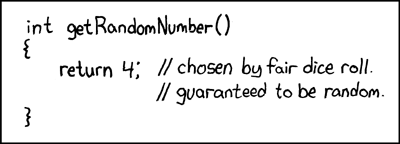
\includegraphics[width=\textwidth]{images/random_number}
}{Randall Munroe, \url{http://xkcd.com/221/}}
% random: http://xkcd.com/221/

This chapter covers the details of the derivation of some equations.



%% Section %%%%%%%%%%%%%%%%%%%%%%%%%%%%%%%%%%%%%%%%%%%%%%%%%
\section{Mathematical proofs}
\label{app:mathProofs}


% ----------------------------------------------------------------------
\subsection{Preliminary observations}

\begin{gather}
	\mathbf{B} : \nabla\overbar{\mathbf{u}} =  - 2 \nu_{SGS} \left[ \mathbf{S} : \mathbf{S}
		+ \mathbf{S} : \Tskew(\mathbf{\nabla\mycdot\mathbf{u}}) \right] 
		\label{eq:lesKEqProductionTermProofTmp03} \\
	\intertext{The contraction of a symmetric and a skew tensor vanishes by definition}
	\underbrace{\Tskew(\mathbf{T})}_{a_{ij}}:\underbrace{\Tsym(\mathbf{T})}_{s_{ij}} \\
	a_{ii} = 0 \\
	a_{ij} = -a_{ji} \\
	\Tskew(\mathbf{T}):\Tsym(\mathbf{T}) = a_{ij} s_{ij} = 0 \\
	\intertext{Thus, the second term in \eqref{eq:lesKEqProductionTermProofTmp03} vanishes.}
	\mathbf{B} : \nabla\overbar{\mathbf{u}} =  - 2 \nu_{SGS} \mathbf{S} : \mathbf{S} 
\end{gather}





%%%%%%%%%%%%%%%%%%%%%%%%%%%%%%%%%%%%%%%%%%%%%%%%%%%%%%%%%%%%%
%% NOMENCLATURE AND BIBLIOGRAPHY
%%%%%%%%%%%%%%%%%%%%%%%%%%%%%%%%%%%%%%%%%%%%%%%%%%%%%%%%%%%%%

\pagestyle{plain}

%% A small distance to the other stuff in the table of contents (toc)
\addtocontents{toc}{\protect\vspace*{\baselineskip}}

%% The Nomenclature
\setlength{\columnsep}{1.5cm}
\renewcommand*{\nompreamble}{\begin{multicols}{2}}
\renewcommand*{\nompostamble}{\end{multicols}}

\printnomenclature  %creates nomenclature section produced by MakeIndex

% D	dimensionless numbers: 		symbol, description, definition
% G	Greek symbols				symbol, description, unit
% L	Latin (Roman) symbols		symbol, description, unit
% X	Other?						symbol, description, unit
% U	subscripts					symbol, description
% S	superscripts				symbol, description
% O	oversymbols					symbol, description


%% The Bibliography
%% ==> You need a file 'literature.bib' for this.
%% ==> You need to run BibTeX for this (Project | Properties... | Uses BibTeX)
%\nocite{*} %Even non-cited BibTeX-Entries will be shown.
%\phantomsection
\bibliographystyle{plainnat} %Style of Bibliography: plain / apalike / amsalpha / ...
%\addcontentsline{toc}{chapter}{Bibliography} %'Bibliography' into toc  % not needed anymore, thanks to tocbibind
\bibliography{thesisBibliography} %You need a file 'thesisBibliography.bib' for this.









%%%%%%%%%%%%%%%%%%%%%%%%%%%%%%%%%%%%%%%%%%%%%%%%%%%%%%%%%%%%%
%% CV & Eidsstattliche Erklaerung
%%%%%%%%%%%%%%%%%%%%%%%%%%%%%%%%%%%%%%%%%%%%%%%%%%%%%%%%%%%%%

% CV and eidesstattliche erklaerung are mandatory.

\pagestyle{empty} %No headings for the first pages.

\chapter*{Curriculum Vitae}
\addcontentsline{toc}{chapter}{About the author}

\setlength\extrarowheight{5pt}

\begin{longtable}[t]{ll}
	\multicolumn{2}{l}{\textbf{\Large Personal Data}} \\
	Name & Dipl.-Ing. Luca Benvenuti \\
	Email & lucabenvenuti@gmail.com \\
	Date of Birth & May $12^{th}$, 1988 \\
	Citizenship & Italy \\
	Parents & Fabrizio Benvenuti, Daniela Zanoni \\
	\vspace*{1ex} \\ 
	\multicolumn{2}{l}{\textbf{\Large Professional Experience}} \\
	2013 - 2016 & Researcher at the Department of Particulate Flow Modelling at \\
				&		Johannes Kepler University in Linz, Austria \\
	2013 		& Site Engineer and Quantity Surveyor, Ferretti International, \\
		 		& LISCO (Libya). \\
	\vspace*{1ex} \\
	\multicolumn{2}{l}{\textbf{\Large Education}} \\
	2013 - 2016 & PhD-Student of Mechatronics (Doktoratstudium) at Johannes \\
				& Kepler University in Linz, Austria \\
	2012 		& Diploma in Civil Engineering (Dipl.-Ing.) at the Politecnico \\
				& of Milano, Italy \\
	2011		& Erasmus in Civil Engineering at the Ecole Special de \\
				& Travaux Publics of Paris, France. \\
	2010 - 2012 & Student of Civil Engineering (Master) at the Politecnico \\
				& of Milano, Italy \\
	2007 - 2010 & Student of Civil Engineering (Bachelor) at the Politecnico \\
				& of Milano, Italy \\				
	2007 		& Matura at the Liceo Bagatta in Desenzano del Garda, Italy \\
	2002 - 2007 & Schulverein at the Liceo Bagatta in Desenzano del Garda, Italy \\	
	\vspace*{1ex} \\
\end{longtable}


\clearpage
\selectlanguage{ngerman}

\chapter*{Eidesstattliche Erklärung\markboth{Eidesstattliche Erklärung}{}\protect\vspace{2cm}}


Ich erkläre an Eides statt, dass ich die vorliegende Dissertation selbstständig und ohne fremde Hilfe verfasst, 
andere als die angegebenen Quellen und Hilfsmittel nicht benutzt bzw. die wörtlich oder sinngemäß entnommenen 
Stellen als solche kenntlich gemacht habe.
Die vorliegende Dissertation ist mit dem elektronisch übermittelten Textdokument identisch.

\vspace{3cm}


%\begin{flushright} {\Large Linz, im November 2011} \end{flushright}
%\begin{flushright} {\Large Linz, \date} \end{flushright}
\begin{flushright} {\Large Linz, \today} \end{flushright}


%\clearpage

\chapter*{Sworn Declaration\markboth{Sworn Declaration}{}\protect\vspace{2cm}}


I hereby declare under oath that the submitted doctoral dissertation has been written solely by me without any outside assistance, 
information other than provided sources or aids have not been used and those used have been fully documented.
The dissertation here present is identical to the electronically transmitted text document.

\vspace{3cm}

\begin{flushright} {\Large Linz, \today} \end{flushright}
 ?


\end{document}
